% Chapter 5

% variables
\newcommand{\pdirfive}{chapters/plots/chapter5}

\chapter{Future prospects}
\label{chapter5}

The results obtained by the NA64 experiment already probe a large fraction of the parameter space of the $\umodel$ model. As shown in the previous chapter many other interesting models, including ALPs, light scalars, and protophobic vector bosons are within the reach of this experiment. In this chapter, we will explore the future prospects for the experiment, by outlining its main goals and the foreseen setup upgrades. We can summarize them in three items:

\begin{itemize}
\item Cover the parameter space in the $\dmyplane$ plane compatible with the observed relic abundance of DM assuming a freeze-out mechanism taking place in the early universe.
\item Probe the region explaining the $\DMX$-anomaly as the emission of a new neutral boson in a nuclear de-excitation.
\item Explore Dark Sector models weakly coupled to muons in a novel setup at CERN M2 beamline, NA64$_{\mu}$.
\end{itemize}

For the case of the invisible mode, where we are mostly limited by the cross-section of production, improvements in the setup are marginal to increase our signal yield, thus we are mostly limited by the number of EOT accumulated. 
A value of $5 \times 10^{12}$ was estimated to cover the parameter space illustrated in Fig.\ref{fig:dm-alpha-excl}. However, an upgrade of the setup is needed to address the background predicted for such a large number of EOT. The dominant source is the electron-hadron interaction upstream the ECAL as seen in Sec.\ref{ch3:sec:bkg:inv}.
In the visible mode, on the other hand, the signal yield is dominated by the suppression of the efficiency caused by the short decay time of the dark mediator. This means that an improved setup can significantly boost the signal yield accessing the parameter space characterized by a large coupling $\epsilon > 10^{-3}$. This would probe completely the $\DMX$ parameter space compatible with the Beryllium anomaly.

For this foreseen upgrade a new Micromegas design is mandatory. In Sec.\ref{ch5:sec:mm-upgrades} we will present the details of these detectors. It was my responsibility to improve both the hardware design and the MM multiplexing map to reduce the redundancy in the case of a double hit. This upgrade will benefit all setups with a decrease in material budget and larger transverse acceptance. Furthermore, a good two hit separation is mandatory to use the MM to reconstruct close ($\sim$\SI{2}{mm})) double hits from the $\DMX \to \ee$ decay. To this aim, the new multiplexing map was capable of providing this level of precision, as detailed in Sec.\ref{ch5:sec:separ-hit-micr}.
In Sec.\ref{ch5:sec:new-invismode-setup}, we will cover the main upgrades for the invisible mode setup. A background estimate for the background expected we performed is also provided. This estimate using the implementation of the Straw tubes in the simulation we developed \cite{pdegen-thesis}. In Sec.\ref{ch5:sec:new-vismode-setup}, we will present the new setup I optimized to cover the remaining region of $\DMX$ parameter space. Moreover, in case signal-like events are observed, the upgraded setup we will be able to reconstruct the invariant mass of the particle decaying after the dump. This will allow unambiguous identification of the X17.
The feasibility study for this new setup was accepted as a CERN preprint \cite{Depero:2020zfy}. Finally, in Sec.\ref{ch5:sec:muon-mode-setup}, we will briefly discuss a new approach, using a high-intensity muon beam to boost the results on $\DM$ for larger masses and to probe additional model, like a $\DMU$ boson interacting via a $L_{\mu} - L_{\tau}$ current.
%----------------------------------------------------------------------------------------

\section{Micromegas upgrade}
\label{ch5:sec:mm-upgrades}

An upgrade of the Micromegas detectors is needed to decrease the material budget and improve the tracking procedure. As seen in chapter \ref{chapter3}, the main background for the invisible mode is caused by electro-nuclear production upstream of the ECAL that causes a large amount of energy to escape transversely. To decrease the chances of these interactions, the material along the beamline has to be minimized. The next Micromegas generation will use a 100 $\mum$ Mylar window to seal the gas box, instead of the thick (\SI{3}{mm})
Copper/PCB seal used in the last design. The PCB on the bottom will also be built using a honeycomb structure of 3 mm and 100 $\mum$ of glass epoxy to connect the PCB to the XY strips. The existing modules are also modified in the same way as shown in Fig.\ref{fig:mm-old-new}. A hole was cut in the copper seal with the same dimension of the active area ($80 \times 80$ $\mms$) and sealed using an aluminized Kapton foil. The advantage of this technique is that the material seals the gas box and applies the voltage needed by the drift simultaneously.

\begin{figure}[bth!]
  \centering
  \includegraphics[width=\textwidth]{\pdirfive/mm-new-old.pdf}
  \caption[Previous version and new Micromegas design of the gas box seal]{Left: Micromegas modules used during 2018 beam time with Epoxy+Copper seal for the gas box. Right: the same module after the seal of the gas box is substituted with an aluminized Kapton foil to decrease the material budget.}
  \label{fig:mm-old-new}
\end{figure}

The performance of the new modules was tested first using a $^{55}$Fe to trigger ionization in the gas chamber and later by using cosmic muons to directly compare the efficiency of both designs. The results in terms of efficiency and uniformity were compatible within $\lesssim$1\%. A small voltage drop along the foil was observed, but not accompanied by a degradation of the efficiency \cite{philip-swork}.

A second upgrade is the production of larger Micromegas modules to increase the acceptance in the bending direction. These new modules will be used in the new setup for the visible mode and in NA64$_{\mu}$ experiment, detailed in Sec.\ref{ch5:sec:new-vismode-setup} and Sec.\ref{ch5:sec:muon-mode-setup} respectively. The modules have an active area of 245$\times$80 $\mms$, with a pitch size of $250$ $\mum$ as in the previous version. Their multiplexing factor will remain 5:  960$\times$80 strips will be read by two APV25 chips, for a total of 256 channels \cite{apv-useguide}. The dimensions were chosen as a compromise between the acceptance and cost-effectiveness of the modules. Using a MC-simulation, it was checked that a length of 245 $\mmi$ is sufficient to reach an acceptance of $\gtrsim$95\% in both visible and muon setup.

The hit resolution is not expected to change as the pitch size is not changed. However, a new multiplex map was developed for both 80$\times$80 $\mms$ and 256$\times$80 $\mms$ Micromegas to further reduce the redundancies and prevent distorted cluster topologies generated by close strips connected to the same channel. The new map for the $80\times80$ $\mms$ Micromegas was improved following the principle to maximize the distance between strips connected to the same channel. In the old mapping, this minimal distance was 3, which caused cluster distortions in specific regions of the plane. In the new mapping, this distance was increased to 16. The new multiplex map for the larger plane was constructed in the same way, with a minimum distance of 24 strips. The complete description of the new maps is given in Appendix.\ref{sec:multiplex-maps}. The maps were also tested using a toy Monte-Carlo based on 2018 data: clusters are generated starting from templates obtained in the calibration run collected at low intensity, and then placed in a random position on the plane. This study revealed an excellent homogeneity of the map as shown in Fig.\ref{fig:mm-mult-study}. The hit residuals, defined as the difference between the true hit position and the reconstructed one using the NA64 cluster finder, was found to be constant along the plane. A more detailed study of the residuals as a function of the distance between hits is presented in Sec.\ref{ch5:sec:separ-hit-micr}.

\begin{figure}
    \centering
    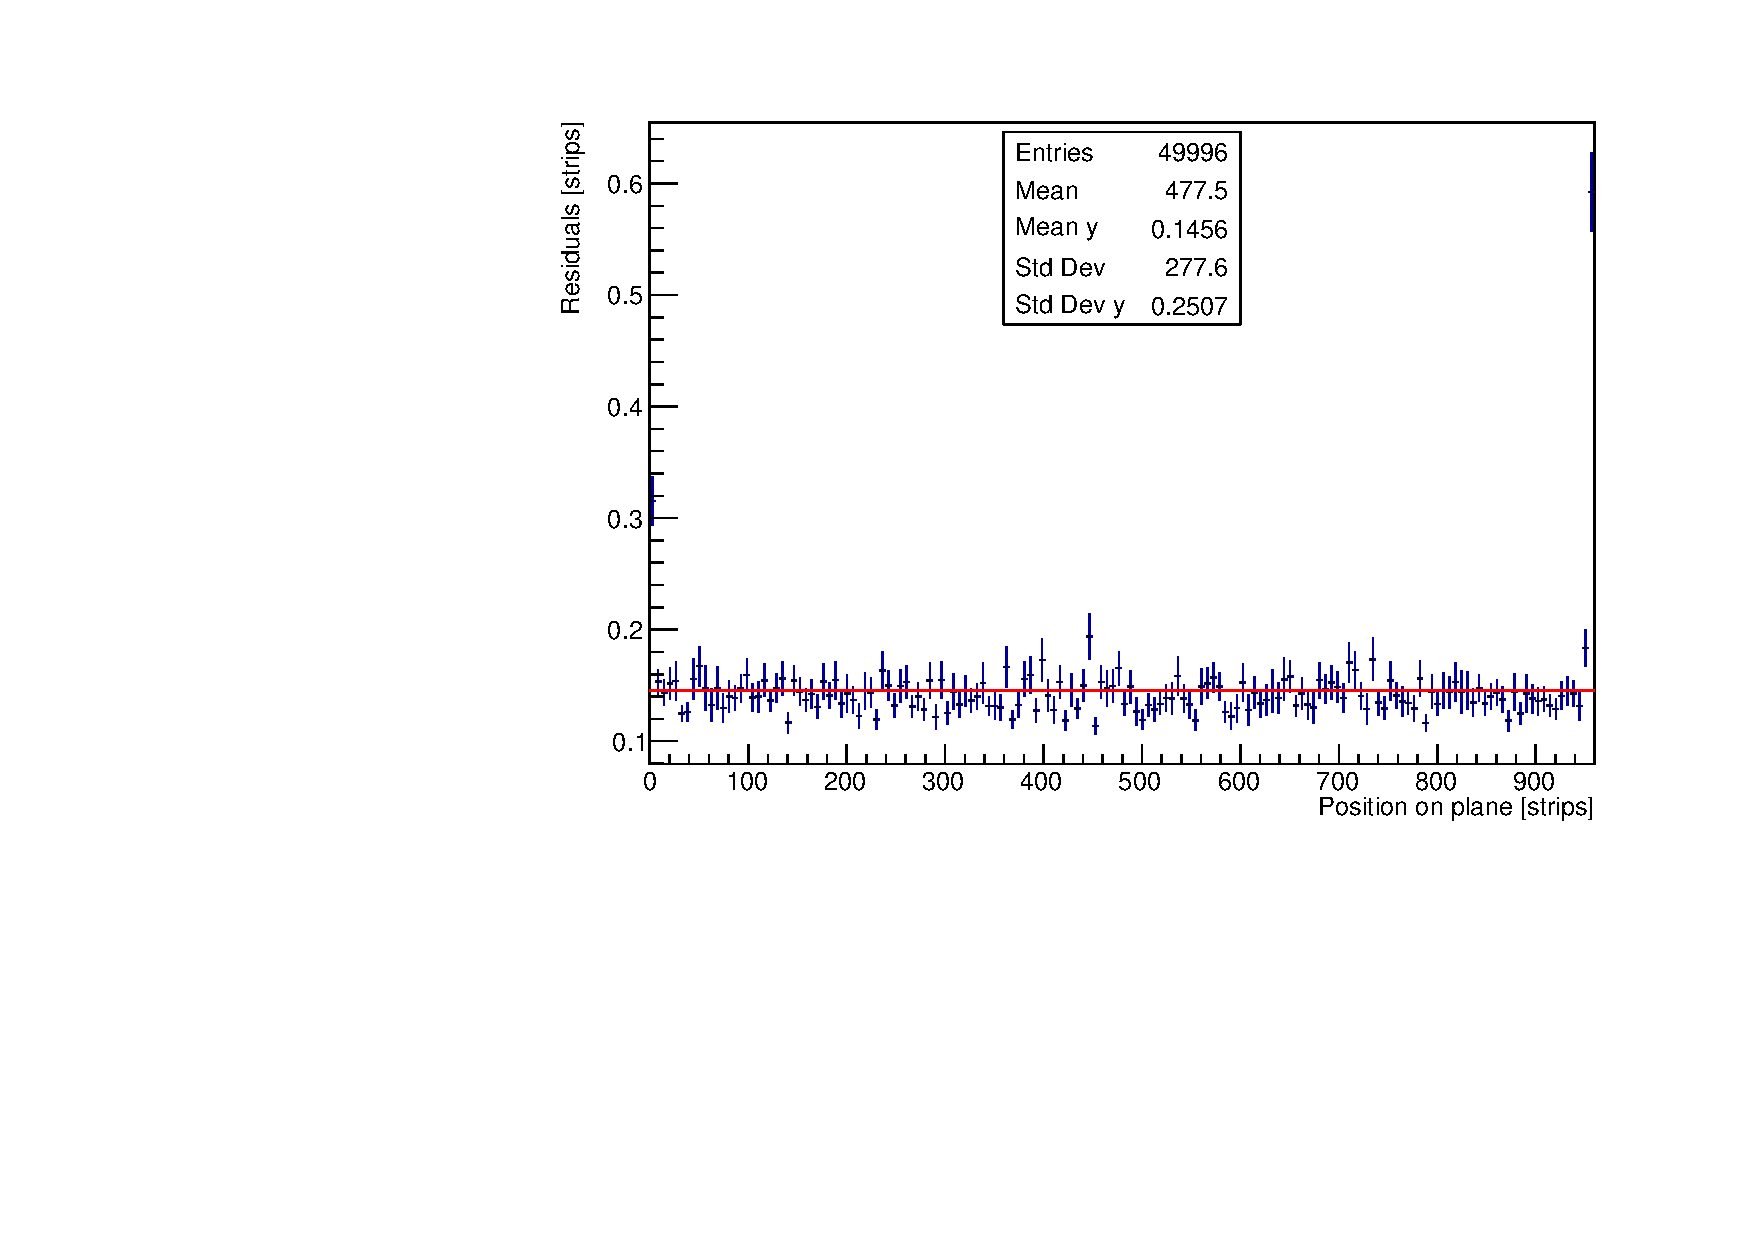
\includegraphics[width=\textwidth]{\pdirfive/residual_cluster1_series1_chan192.pdf}
    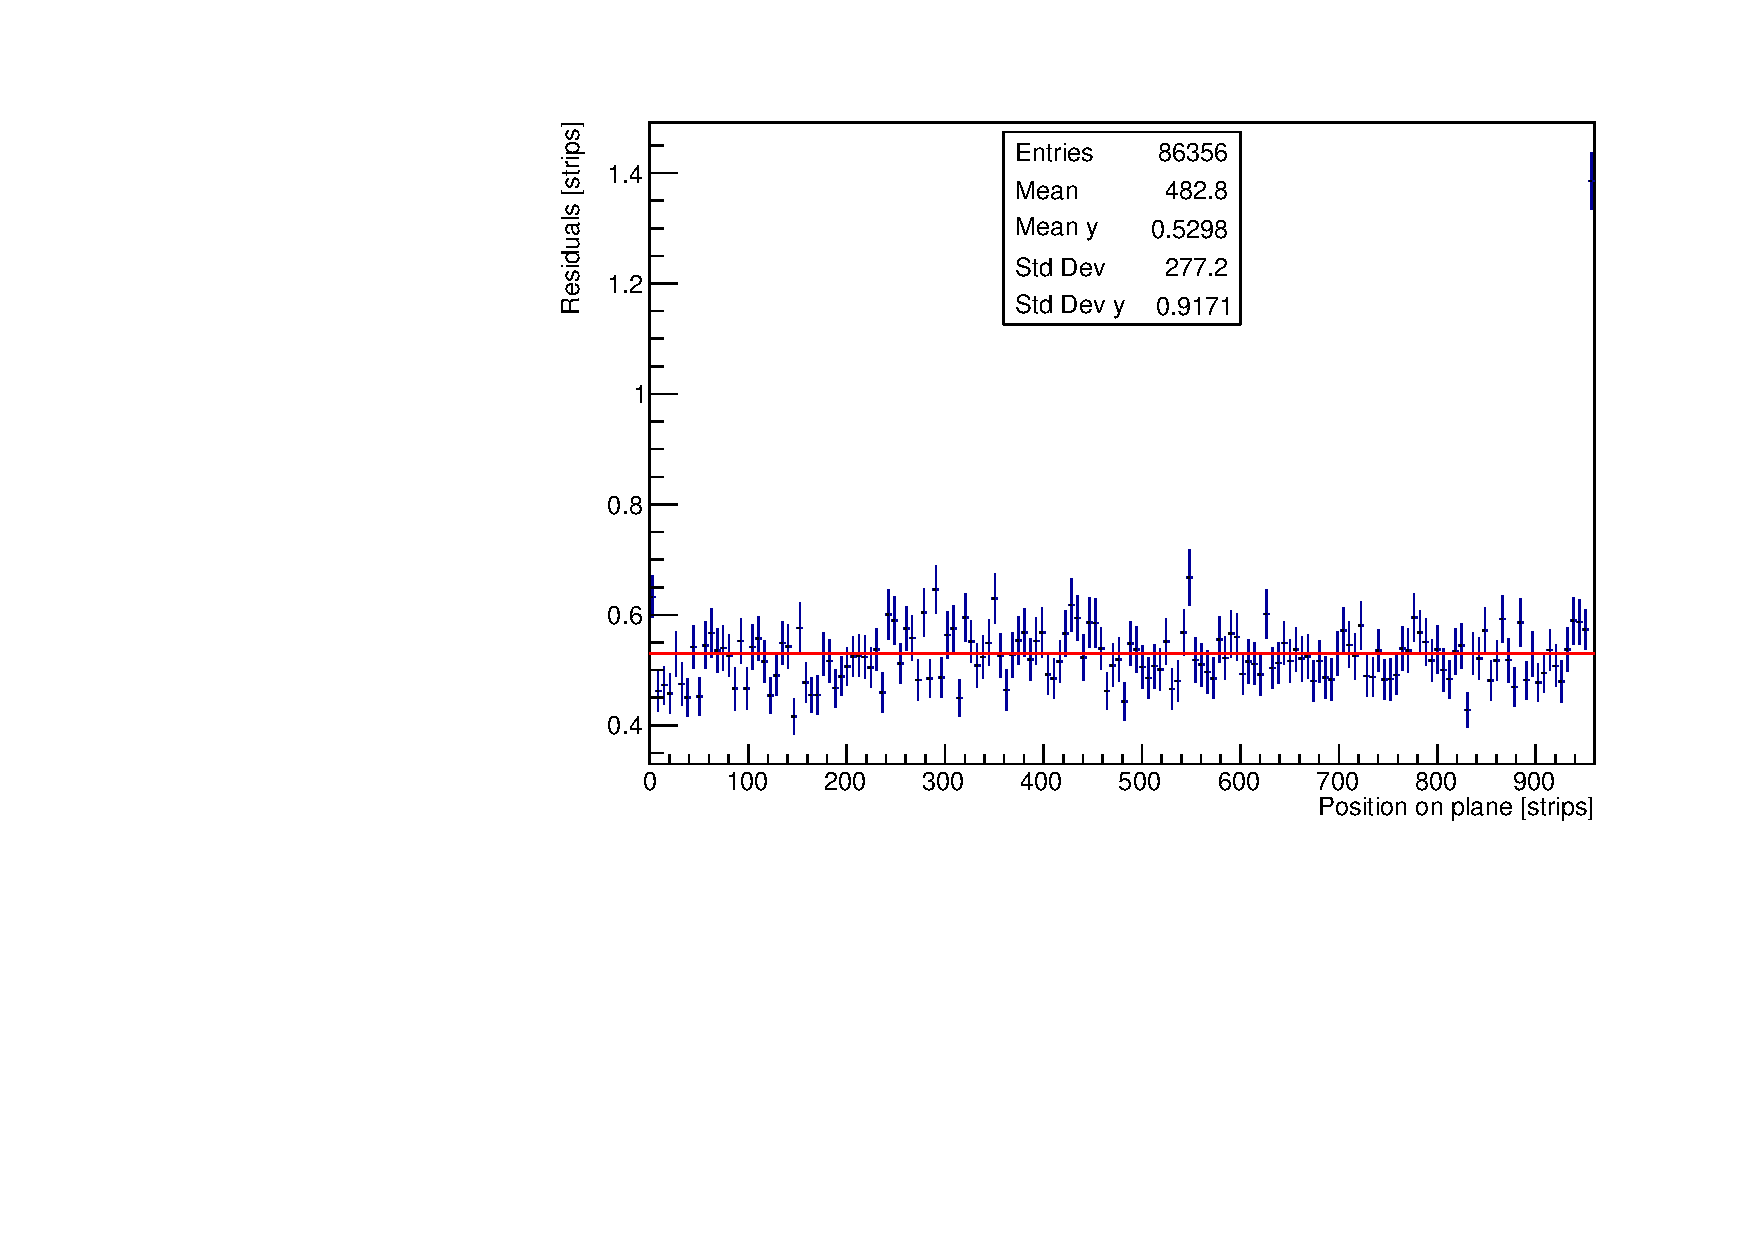
\includegraphics[width=\textwidth]{\pdirfive/residual_cluster2_series1_chan192.pdf}
    \caption[Test of new multiplex map]{Simulated residual of the reconstructed hit position as function of the primary impact point on a Micromegas plane. The new multiplexed map generated for the 245$\times$80 $\mms$ generates the plane output. The residuals are presented for a single cluster (top) and for two clusters (bottom).}
    \label{fig:mm-mult-study}
\end{figure}


\FloatBarrier\noindent
\section{Improvement to the invisible mode setup}
\label{ch5:sec:new-invismode-setup}

Increasing the statistics is the goal for the next 2021 invisible mode runs to probe the region of parameter space compatible with the observed relic density in a freeze-out scenario. It is estimated that 5$\times 10^{12}$ EOT are needed for this purpose, as can be seen in the projection shown in Fig.\ref{fig:dm-sens-proj}.

\begin{figure}[bht!]
  \centering
  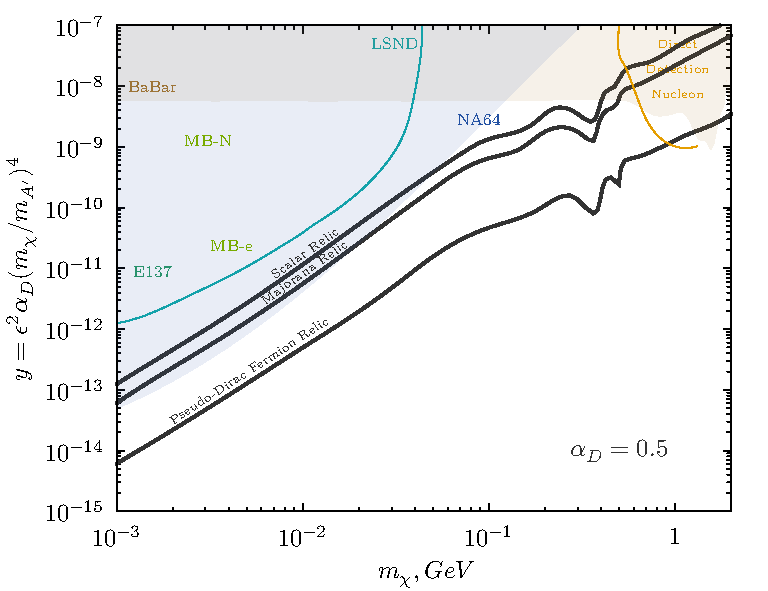
\includegraphics[width=0.45\textwidth]{\pdirfive/tldra-19-2-alpha_0_5.pdf}
  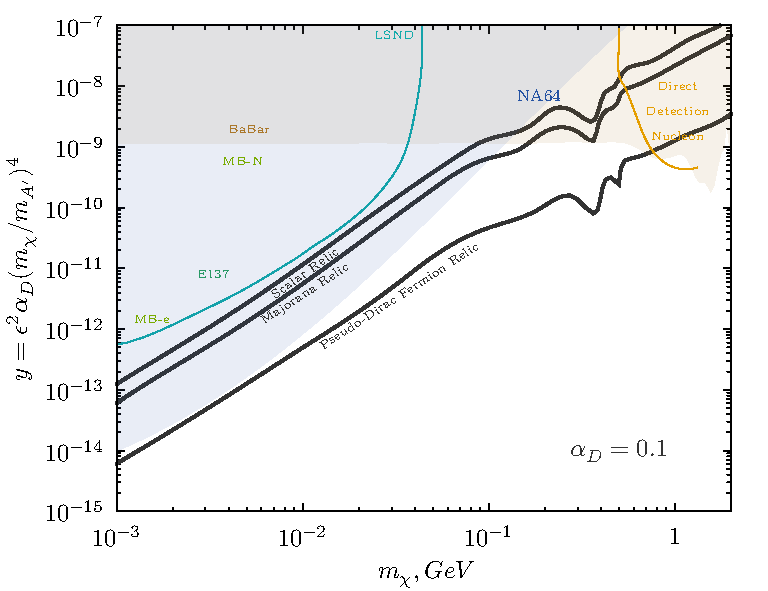
\includegraphics[width=0.45\textwidth]{\pdirfive/tldra-19-2-alpha_0_1.pdf}
  \caption[Sensitivity projection for invisible mode 2021]{Limits on the $\dmplane$ plane assuming a number of EOT collected of 5$\times 10^{12}$ by extrapolation of the results obtained using 2016-2018 data set. The favored parameters to account for the observed relic DM density for the scalar, pseudo-Dirac and Majorana type of light DM are shown.}
  \label{fig:dm-sens-proj}
\end{figure}

For this large statistic, the main problem is the background.  We saw in chapter \ref{chapter3} that the dominant contribution comes from electro-nuclear scattering in the beamline before the target. In this section, we study this source in detail and estimate its contribution to the expected larger sample.

In Fig.\ref{fig:enucl-position} we see the frequency of nuclear interactions for different positions along the beam-line predicted from a dedicated MC-simulation. Micromegas detectors are the leading contribution to this background, as a result of their large budget material, which in terms of interaction lengths is approximate $\lambda_{int} \simeq 1.9 \times 10^{-3}$. However, a factor $\sim 2$ less electro-nuclear interaction is observed in MM$_3$. This is the result of the thinner material of this module, which uses a Mylar window instead of a Copper one to close the gas box. The substitution of the gas box cover for the rest of the modules will be an important improvement to suppress this background, already discussed in Sec.\ref{ch5:sec:mm-upgrades}. To reduce it further, the transverse coverage of the setup needs to be increased. Naively this can be done by increasing the size of the HCAL, but this solution is rather expensive as it would require a very large module. Instead, a new detector called VHCAL\footnote{Veto Hadronic Calorimeter} is used for the same purpose. This detector is a Copper-scintillator sandwich calorimeter with a hole in the middle to remove the material in the way of the beam and a lateral size of $50\times50$ \si{\centi\meter\squared}. It will be located upstream of the ECAL just after the first tracking detectors as shown in Fig.\ref{fig:vhcal}.
\begin{figure}[bth!]
  \centering
  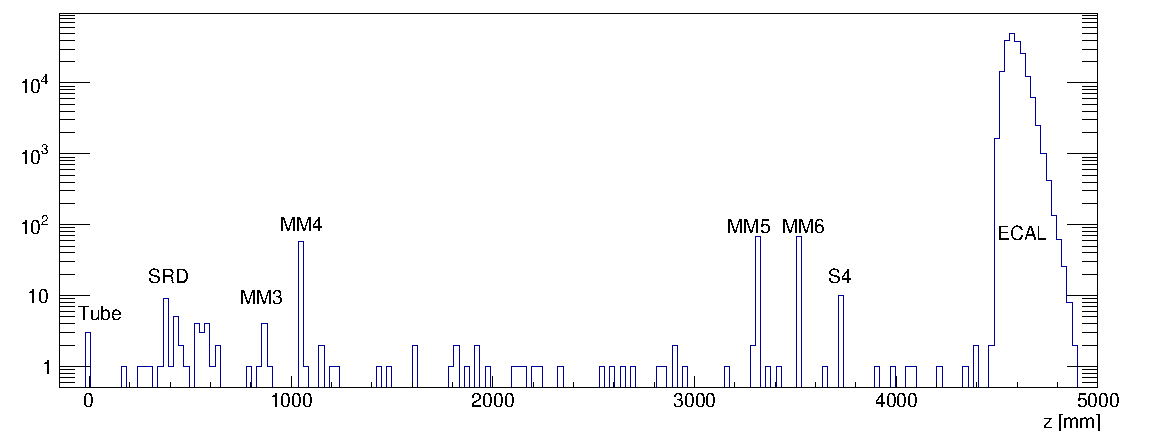
\includegraphics[width=\textwidth]{\pdirfive/enucl-position.pdf}
  \caption[electro-nuclear interaction position]{Z position of electro-nuclear interactions between the end of the vacuum tube and the start of the first HCAL. A total of 2.5$\times 10^6$ EOT were simulated for this distribution.}
  \label{fig:enucl-position}
\end{figure}

\begin{figure}[bth!]
  \centering
  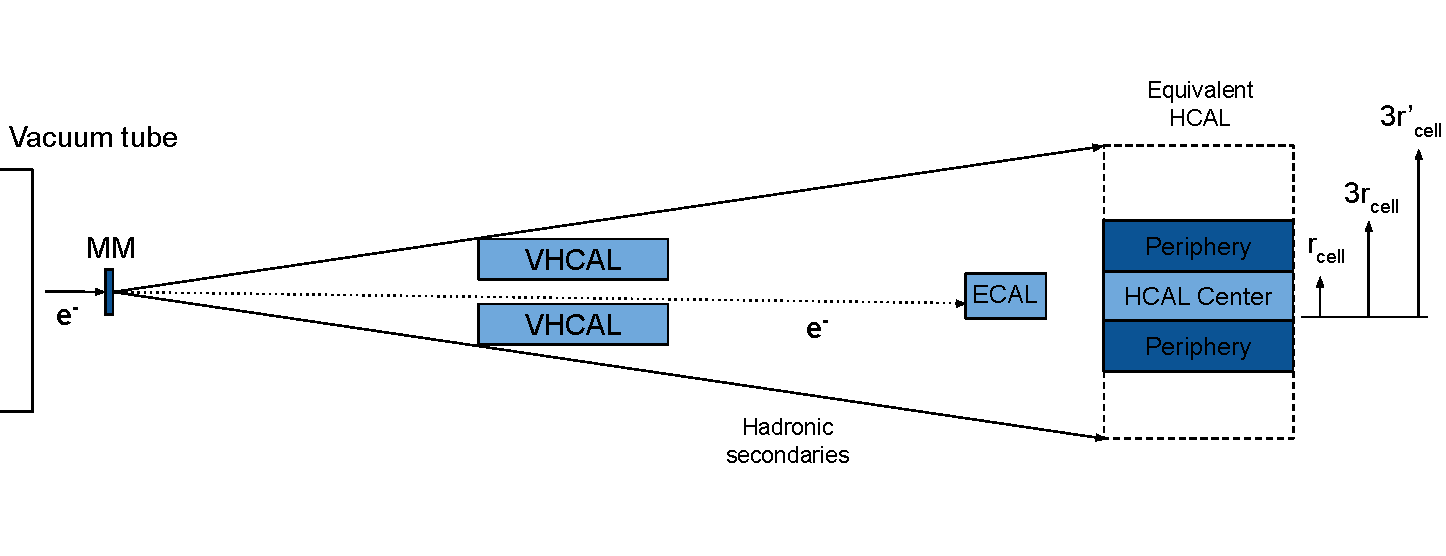
\includegraphics[width=\textwidth]{\pdirfive/VHCAL.pdf}
  \caption[Sketch of VHCAL in invisible mode setup 2021]{Sketch of the VHCAL in the 2021 invisible mode setup. Coverage of large angle particle scattering is shown, together with the equivalent size of the HCAL in this arrangement.}
  \label{fig:vhcal}
\end{figure}

To properly account for this background, we follow the procedure described in \cite{na64-neutrals-study,pdegen-thesis}, reviewed here.
First, we split the $\ehcalplane$ in 10 different zones as depicted in Fig.\ref{fig:enucl-bkg-estimation}. The zones divide the distribution of observed events in several tiles at different distances from the signal region. All the regions labeled with even numbers are events where the energy is conserved and the $R$ value\footnote{Defined as the ratio of the energy deposited in the outer cells with the total energy deposited (see Eq.\ref{eq:R-factor}).} is small (Region II in Fig.\ref{fig:r-value-csample}). In events inside the zones labeled with an odd number, on the other hand, some energy is missing from the initial primary electron. The two most relevant sets are 7) and 9), which include a part of the signal region. These events have an $R$ distribution by average larger, with a sharp peak at 1 (Region III in Fig.\ref{fig:r-value-csample}). To further classify the events, we construct a new category based on the value of $R$. We define $n_i(r)$ as the number of events in the region $i$ with distance $r$ from the center of the HCAL. We can define three categories:

\begin{itemize}
\item $n_{5,7}(r=0)$ number of events with energy deposited in the HCAL.
\item $n_{5,7}(r=r_{cell})$ number of events with $R=1$, i.e. no energy is deposited in the central cell of the HCAL.
\item $n_{5,7}(r=3r_{cell})$ events where particles are emitted outside the HCAL and $R$ is not defined.
\end{itemize}

The final goal is to calculate the probability of an incoming primary electron to produce an event that fall in one of the above categories:

\begin{equation}
  \label{eq:enucl-prob}
  p_i = \frac{n_i(r)}{n_{EOT}}
\end{equation}

In practice, the distribution of $n_{i}(r)$ is fitted using an exponential integrated in the region $n_i(r>r_{cell})$ relevant for the background. For an arbitrary number of EOT, we use the equation:
\begin{equation}
  \label{eq:exp-bkg-inv-2021}
  n^{bkg}_i \simeq n_{EOT} \times p_i(\lambda \times r)
\end{equation}
where $\lambda = r'_{cell}/r_{cell}$ is a scale factor. In our case we set $n_{EOT} = 5 \times 10^{12}$, $r_{cell}$ as the total radius covered in 2018 and $r'_{cell}$ as the equivalent cell radius that will be covered in 2021. Assuming a VHCAL placed at 3 \si{\meter} distance from the ECAL, the coverage would roughly amount to an HCAL with three times its current transverse size, thus $\lambda = 3$. We evaluate the fit $p_i(r)$ for the zones 7 and 9 relevant for our signal region using these values. The current best estimate for this background is 5$\pm$3 events after taking into account the reduced material budget of the Micromegas \cite{pdegen-thesis}. The background extrapolation is illustrated in Fig.\ref{fig:enucl-bkg-extrapolation} comparing MC and data for both regions.


\begin{figure}[tbh!]
  \centering
  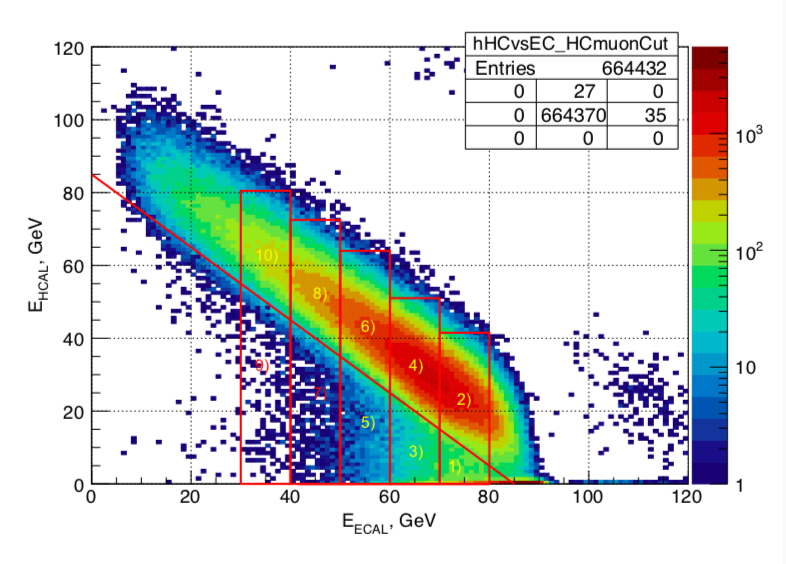
\includegraphics[width=0.45\textwidth]{\pdirfive/zones-no-veto.png}
  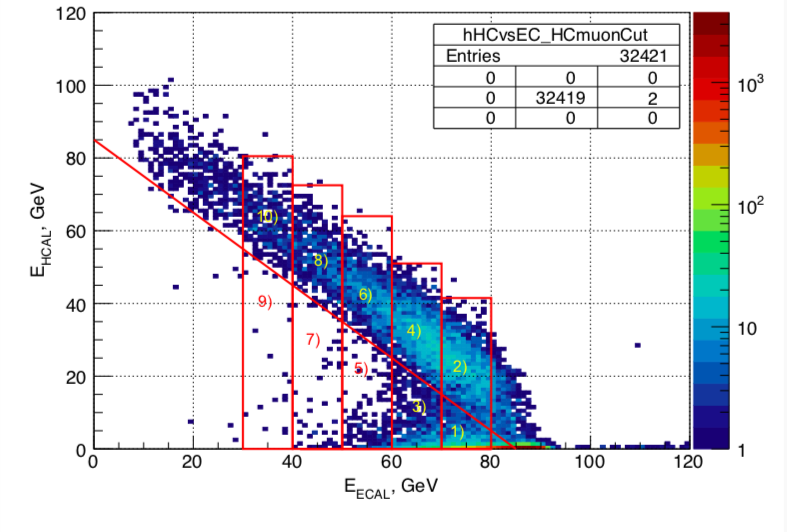
\includegraphics[width=0.45\textwidth]{\pdirfive/zones-veto.png}
  \caption[Electro-nuclear background estimation]{Division of the $\ehcalplane$ plane in ten zones for background estimation. The left panel shows the control sample of events after using SRD, tracking, pileup-removal and a hit in the central cell of the ECAL as selection criteria. The right panel shows the same sample after the events with signal in the VETO counter are removed. Adapted from \cite{na64-neutrals-study}.}
  \label{fig:enucl-bkg-estimation}
\end{figure}

\begin{figure}[bth!]
  \centering
  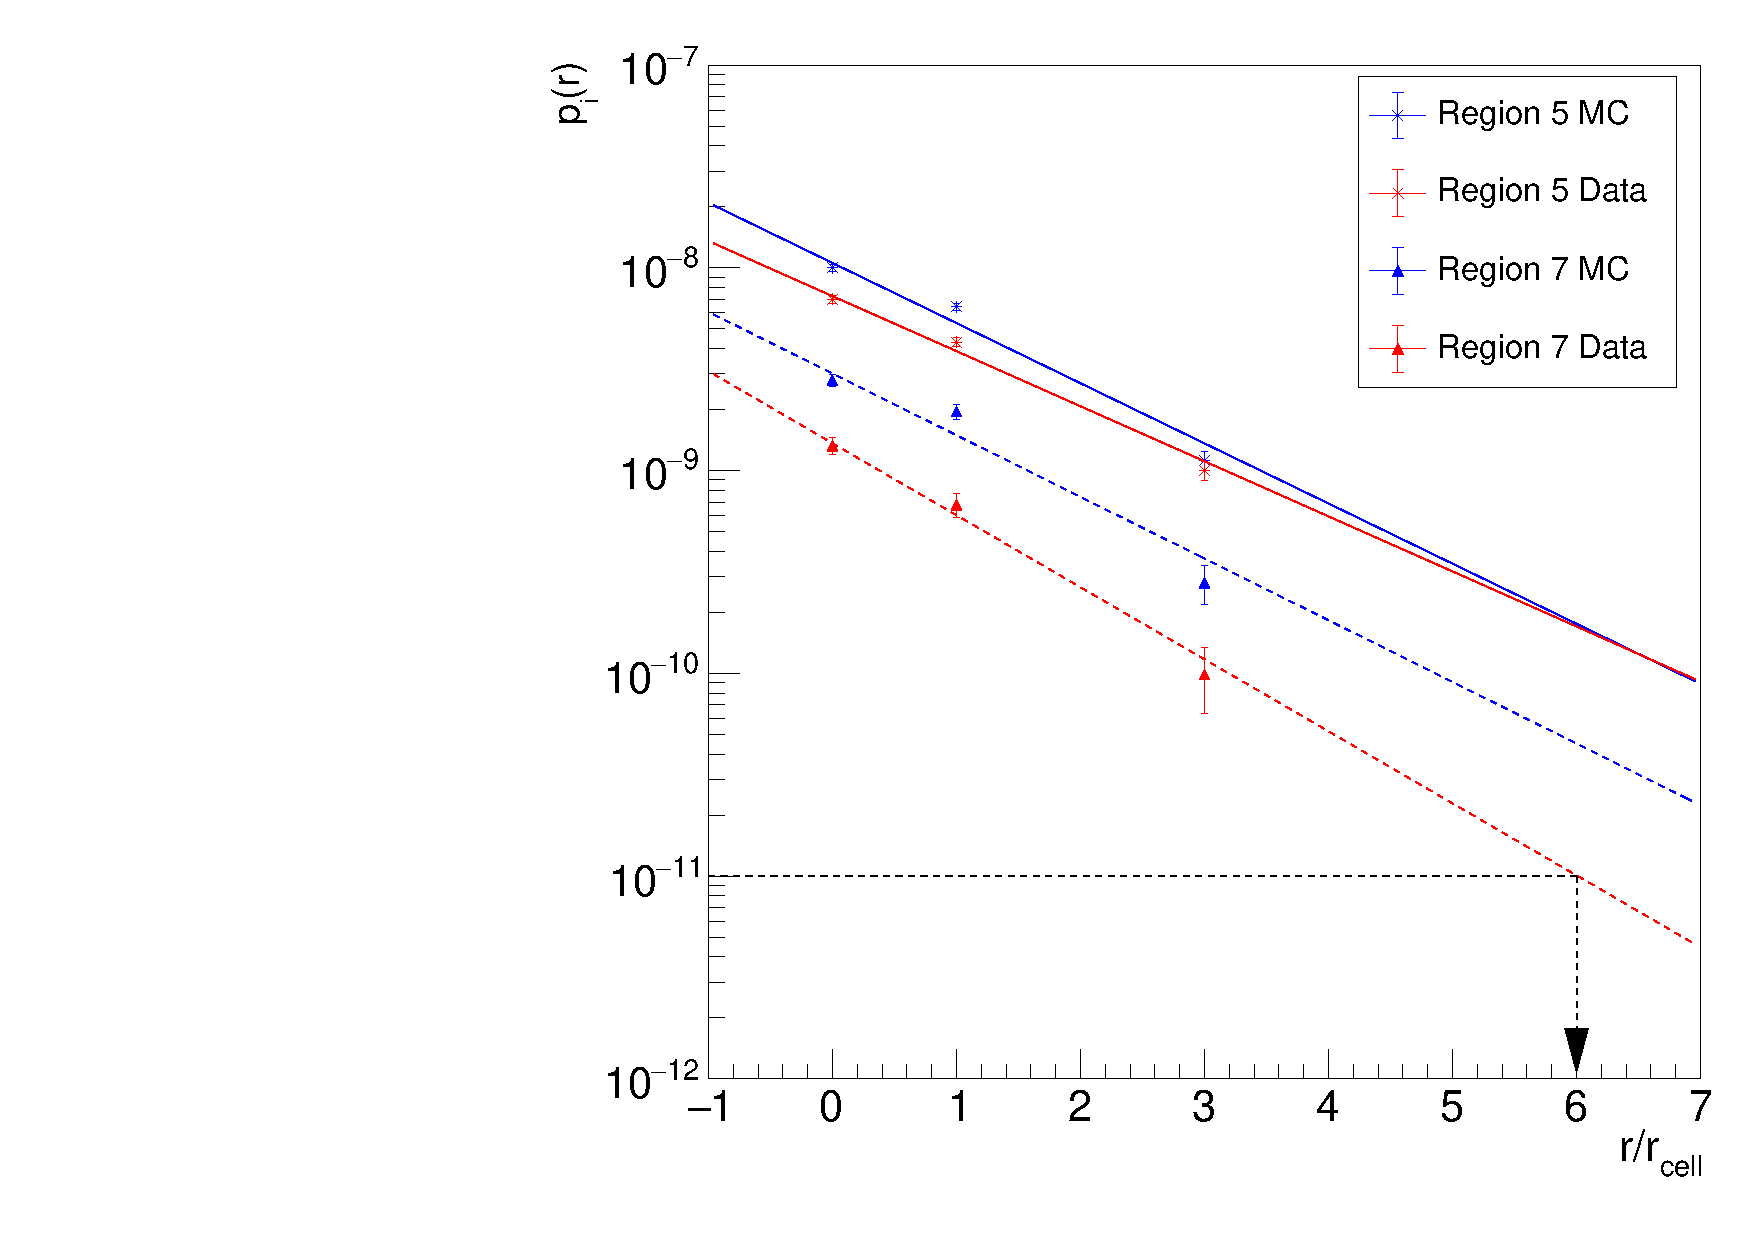
\includegraphics[width=0.7\textwidth]{\pdirfive/pp999-bkg-p.pdf}
  \caption[Background extrapolation invisible mode]{Probability of missing energy event as a function of the HCAL transverse size. Extrapolation is performed for both MC and data for region 5 (continuous line) and region 7 (dashed line) as illustrated in Fig.\ref{fig:enucl-bkg-estimation}.}
  \label{fig:enucl-bkg-extrapolation}
\end{figure}

\clearpage

\section{Improvement to the visible mode setup}
\label{ch5:sec:new-vismode-setup}

The main goal of the visible mode data taking in 2021 will be to probe the remaining parameter space that justifies the $\DMX$-anomaly. In chapter \ref{chapter1} we gave an overview of the possible models, and in chapter \ref{chapter4} we have shown that in the case of a protophobic vector boson the data collected by NA64 constraints the possible couplings to $6.8 \times 10^{-4} < \epsilon < 1.4 \times 10^{-3}$. The mass of $\DMX$ can also be calculated with high precision by fitting the nuclear spectrum of the anomaly. This procedure currently gives compatible results for the two atoms studied, claiming a mass of 16.70$\pm$0.85 $\mev$ for Beryllium and a mass 16.84$\pm$0.36 $\mev$ for Helium. The current setup is unable to probe this particle, as the analysis of the visible mode data has shown. The remaining region of parameter space $6.8 \times 10^{-4} < \epsilon < 1.4 \times 10^{-3}$ is extremely challenging to probe in the current setup. The reason for this is the high coupling of this region suppresses exponentially the signal yield due to the short decay length. We can observe this by inverting Eq.\ref{eq:dm-rate-vis} and transform it into an expression to probe different values of $\epsilon$. If we define $\epsilon_{\textrm{up}}$ as the maximum $\epsilon$ that can be probed with a given set of data and we absorb all the constant in $C'$ we find:

\begin{equation}
  \label{eq:x17-coverage}
  \epsilon_{\textrm{up}} \sim C' \times \frac{E_0}{L_{\textrm{dump}}m^2_{\DMX}} \times \ln{\left(N_{EOT} \epsilon^2 \frac{m_e^2}{m_{\DMX}^2}\right)}
\end{equation}

Increasing the number of EOT only improves our limit logarithmically, and a quick computation shows that an unfeasible number $>10^{14}$ events is needed to explore this region. A new setup was proposed to increase the signal yield while keeping the background under control by decreasing the length of the target. The main limitations come from the short decay length of the $\DMX$ and the difficulty to separate the $\ee$ using trackers. The desired setup will need to boost the signal detection efficiency to a level where the $\DMX$ can be searched for with a realistic number of EOT. Moreover, to unambiguously identify the X17 a spectrometer is added to the setup in order to measure precisely the invariant mass of the $\xdecay$ decay. In summary, we need to address the following aspects:

\begin{itemize}
\item Increase the probability of the $\DMX$ to exit the dump up to at least 20\%.
\item Enlarge the distance between the trackers and the decay base of the $\DMX$ to allow the separation of the $\ee$ pair by at least a few mm.
\item Allow the momentum reconstruction of the $\ee$ pair in the $\xdecay$ decay with an accuracy of $\sim$1\%.
\end{itemize}

In the following sections, we will explore these issues, and provide a solution for each of them in the new setup design. Finally, we estimate the projected  EOT and the time needed to cover the anomaly completely.

\subsection{Invariant mass reconstruction}
\label{ch5:sec:new-vismode-setup-invmass}

The novel setup proposed for 2021 aims to further improve the background suppression and add the full invariant mass reconstruction for the decay of a very short-lived particle generated at the beginning of the dump. In this section, the reconstruction technique is illustrated and the main challenges are outlined. A study based on a full MC simulation of the setup is used to demonstrate the power of the method and its capability of probing the parameter space left to justify the $\DM$ anomaly.

The remained unconstrained parameter space for the coupling $\epsilon$ corresponds to an extremely short-lived $\DM$ with the lifetime $\tau_{\DM} \lesssim 10^{-13}$ s. In chapter \ref{chapter1} we computed the decay length in Eq.\ref{eq:dm-decay-length} as a function of the coupling $\epsilon$, the mass of the mediator, and its energy at the time of emission.
We observe that the $\DMX$ requires energy of $\gtrsim$100 $\gev$ to have a 30 mm decay length comparable to the dimension of the dump.
Additionally, as $E_{\DMX} \gg \mee$, the minimal $\ee$ opening angle and the invariant mass are given by
\begin{equation} 
\angee^{min} \simeq  \frac{2\mee}{E_{\DMX}},
\label{eqn:angle}
\end{equation}
\begin{equation}
\mee = [E_{e^+} E_{e^-}]^{1/2} \angee
\label{eqn:imass}
\end{equation}

For an energy $\sim$100 \gev, the average angle is $\sim$0.34 mrad, which is challenging to be measured with precision $\lesssim 10\%$. Instead, we use the short decay length to fix the vertex position of the $\xdecay$ decay and we reconstruct $\angee$ from the separation of the $\ee$ pair in the trackers placed downstream. As the $\DMX$ is a short-lived particle, its decay vertex $Z_{\DMX}$ is located at the vicinity of the WCAL $Z_{WC}$. This means that $Z_{\DMX} \simeq Z_{WC} \ll L_D$ where $L_D=Z_{T1}-Z_{\DMX}$ is the distance from the decay vertex and the first tracking detector (see Fig.\ref{fig:imass_sketch}). Since $L_D \simeq Z_{T1} - Z_{WC}$, the opening angle $\angee$ can be evaluated as 
\begin{equation}
\angee \simeq \arctan{\frac{ L_{\ee}}{L_D}}
\label{angle-est}
\end{equation}
where $L_{\ee}$ is the distance of the $\ee$ pair in the T1 plane. Using error propagation, we can estimate the uncertainty on the angle:

\begin{equation}
  \sigma^2_{\angee} \simeq (\sigma_{L_{\ee}}  / L_D)^2 + (\sigma_{L_D} / L_D)^2(L_{\ee} / L_D)^2,
  \label{eqn:thetaerr}
\end{equation}

where $\sigma_{L_{\ee}}$ is the hit resolution of the tracker and $\sigma_{L_D}$ is the error of the decay base. In our conditions, the second term is negligible due to the high precision of our tracking detectors and the large distance between them and the target. The formula above shows that a distance of $\sim$10 m is sufficient to reconstruct the invariant mass with a precision $\lesssim$10\%. However, this estimate is flawed by the fact that hit resolution worsens as the two hits are closer.

\begin{figure}[bth!]
  \centering
  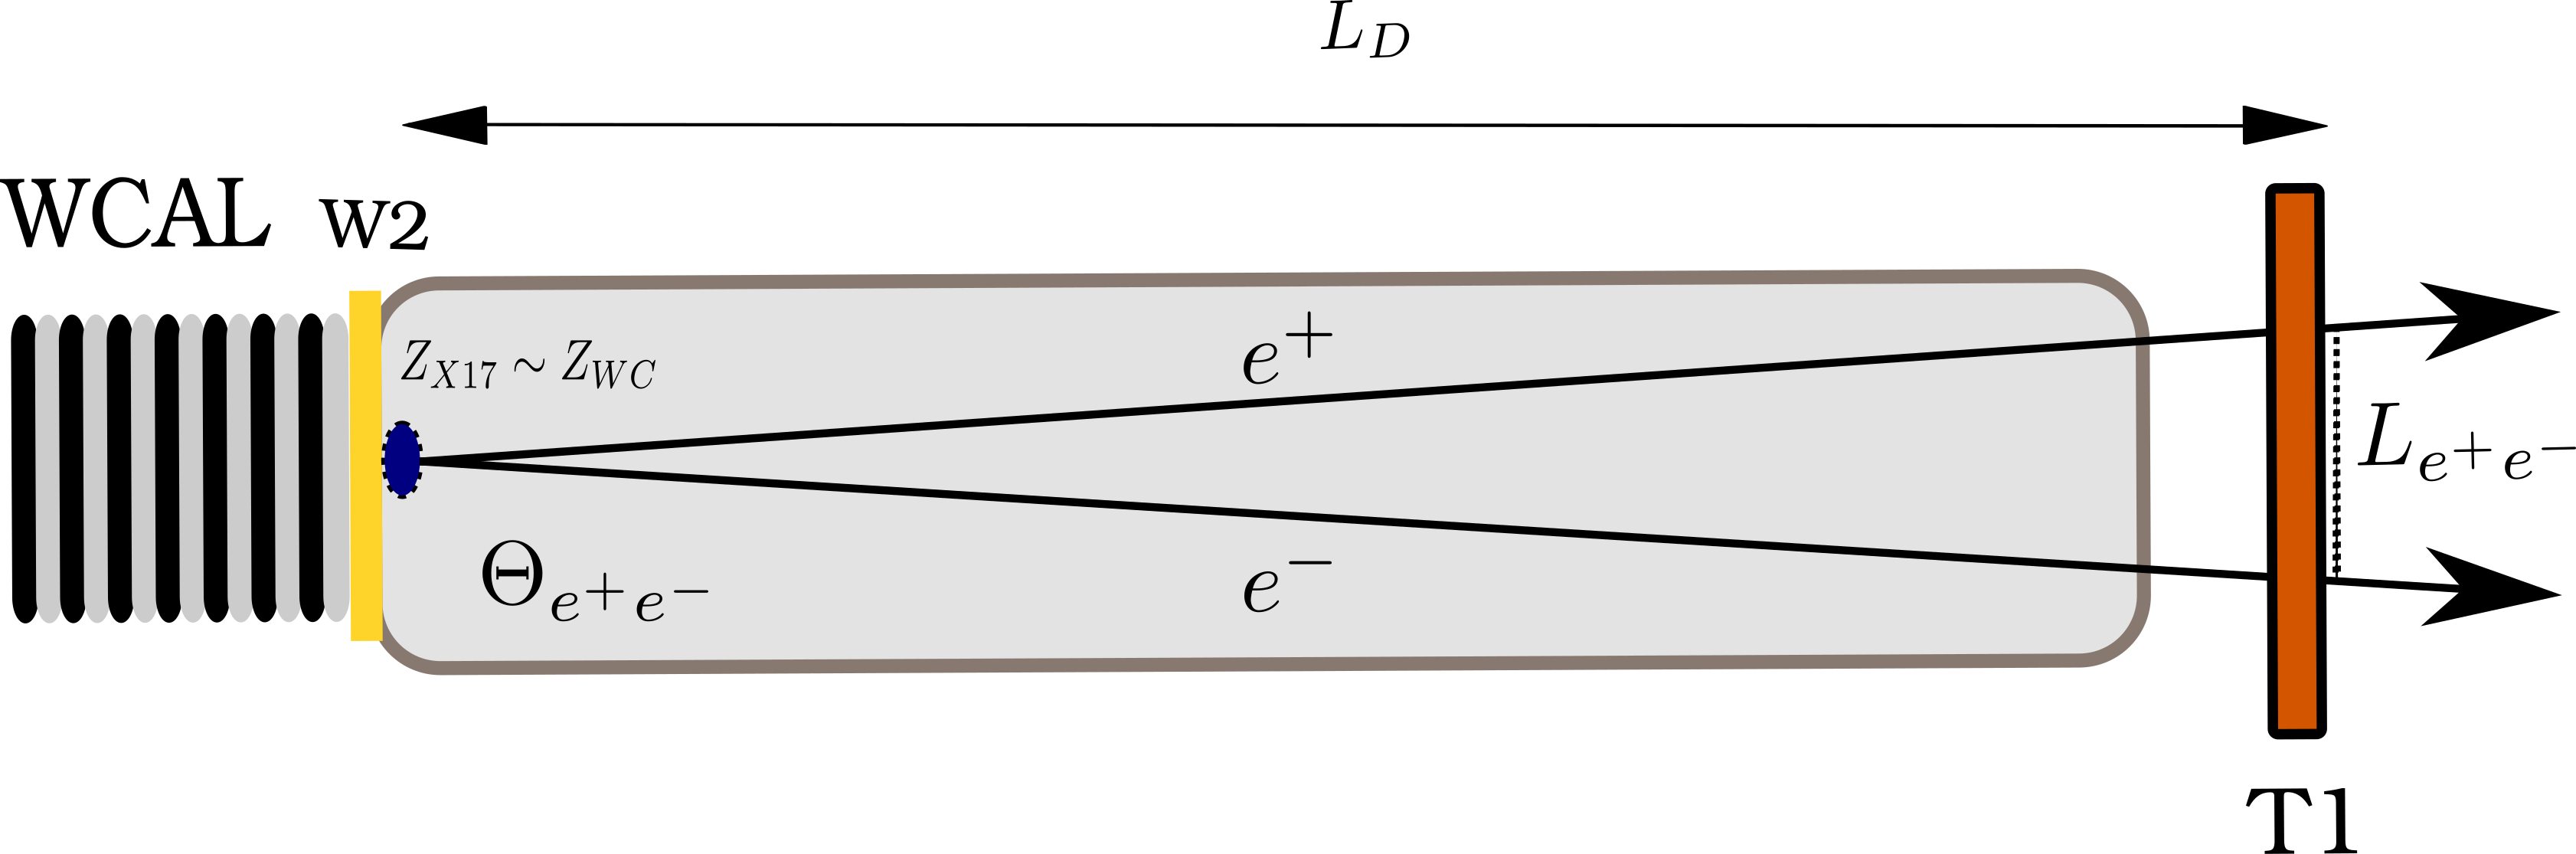
\includegraphics[width=\textwidth]{\pdirfive/imass_sketch.png}
  \caption[Invariant mass reconstruction sketch]{Sketch of the $\DMX$ decay in the proposed setup along the beam axis.}
  \label{fig:imass_sketch}
\end{figure}


This problem has been studied using both fitting procedures and neural networks to reconstruct the original hit position from two overlapped clusters. The data recorded with the trackers during past NA64 runs were used to build a set of different possible topologies. A new set to test different algorithms was then created by mixing these clusters randomly. An example of such a study, where the two clusters are separated using a global fit of two Gaussian is presented in Sec.\ref{ch5:sec:separ-hit-micr}. Both procedures agree that the hit resolution worsens to a maximum of \SI{200}{\micro\meter} when the separation is lower than \SI{1.5}{mm}. No significant worsening in the resolution is observed when the distance between hits exceeds $\sim$2 $\mmi$. In the proposed setup, a distance of \SI{18}{m} is used between the dump and the first tracker, getting an average separation of \SI{5.5}{mm} (Fig.\ref{fig:dm_dist1}). As our data-driven studies have shown, the hits should be well separated in each signal event, granting a hit resolution of \SI{80}{\micro\meter} for the $\ee$ pair.

\begin{figure}[tbh!]
  \centering
  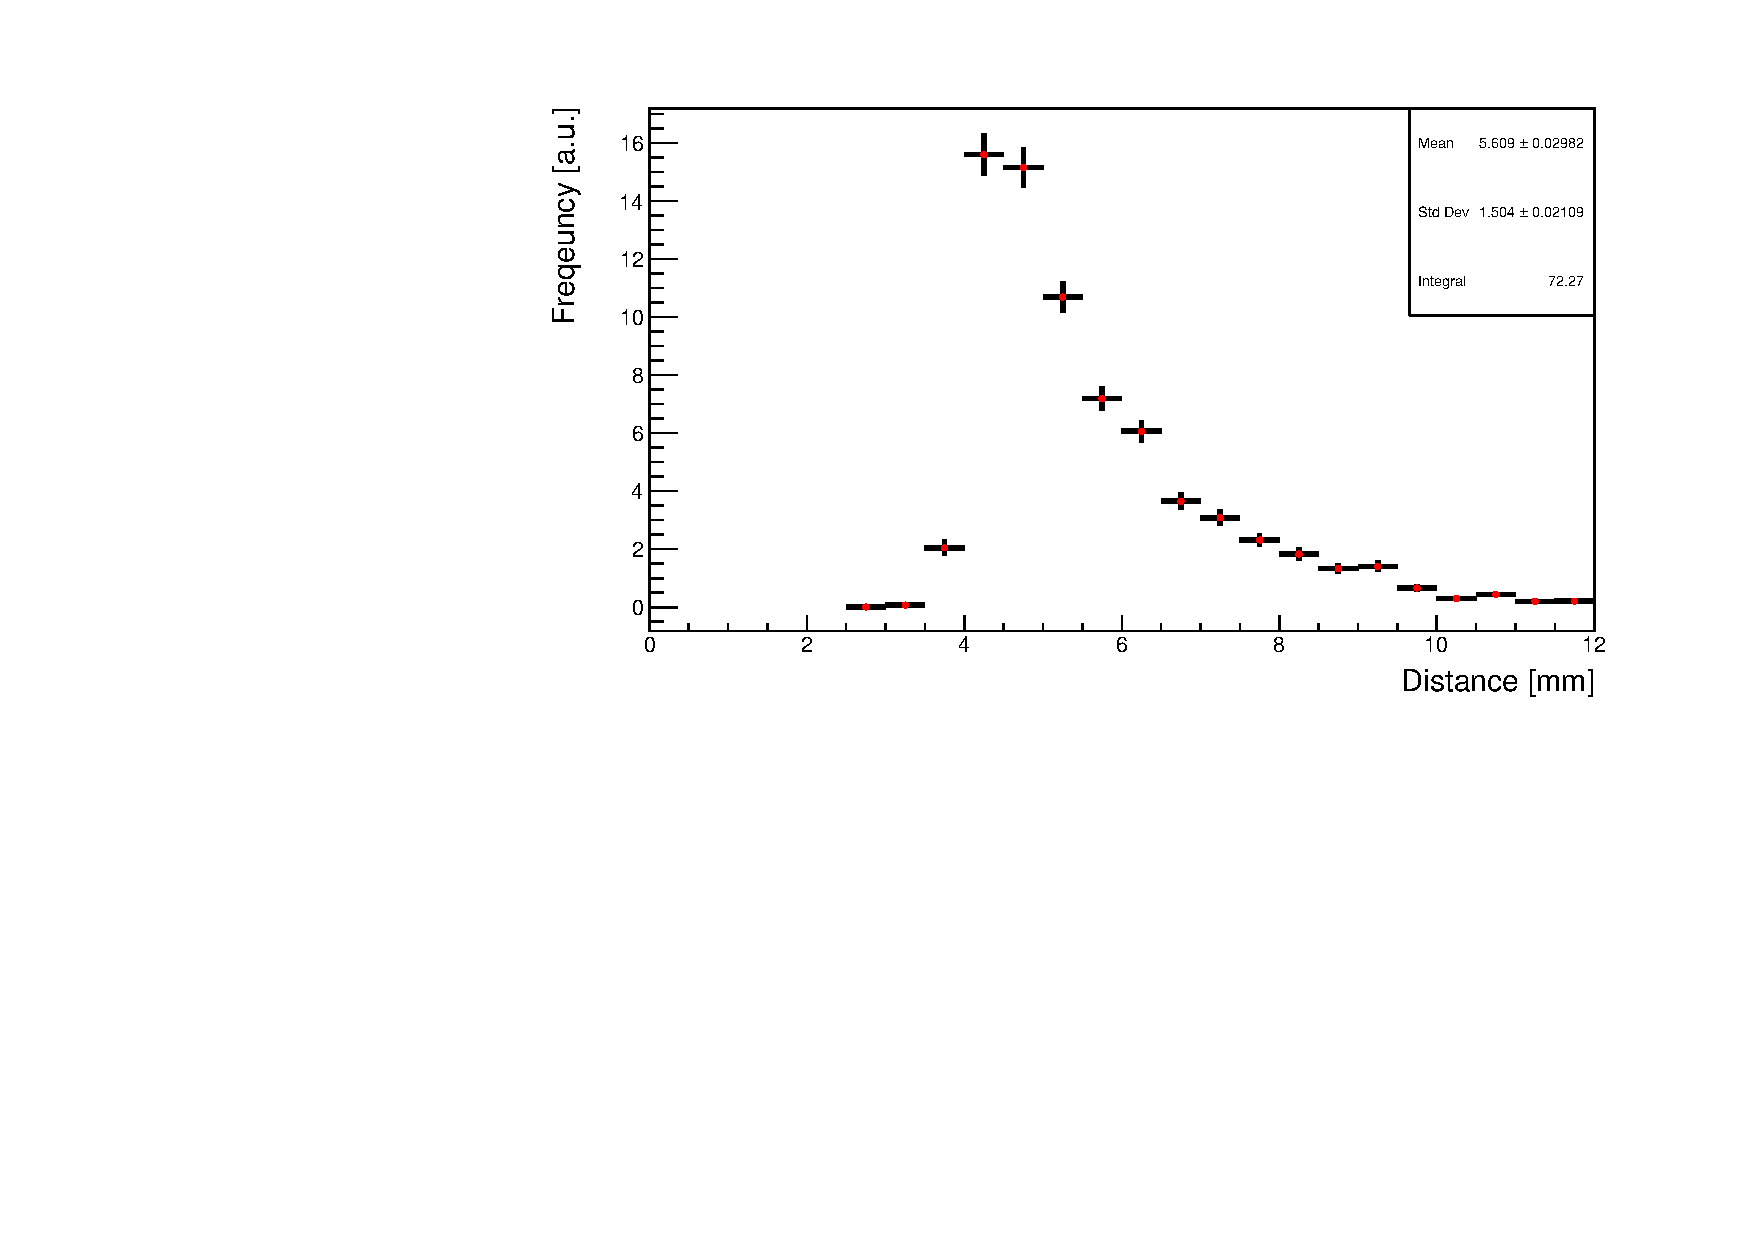
\includegraphics[width=\textwidth]{\pdirfive/DM-dist.pdf}
  \caption[Distance of the decay products of X17 in the 2021 setup]{Distance between decay products of an $\DMX$ decay outside the dump at a distance of 18 m from the decay vertex.}
  \label{fig:dm_dist1}
\end{figure}

To complete the invariant mass reconstruction one needs to know with high precision the momentum of the decay products in a signal-like event. Two independent measurements are used for this purpose. The first one is the momentum reconstruction of the two tracks after passing through a magnetic field. The second one is the measurement of the same two tracks energy in two well-separated em-showers in the ECAL downstream. A dipole magnet bends the two tracks and separates them to reconstruct their energy with a precision of 10\%$/\sqrt{\gev}$ in the ECAL. To achieve this purpose a separation of at least two ECAL cells ($\sim 8$ \si{\centi\meter}) is needed.

The setup proposed uses an \SI{18}{\meter} vacuum tube kept at a pressure of 8$\times 10^{-4}$ \si{\milli\bar}. Two GEM trackers \cite{gem} are placed at a distance of \SI{0.1}{\meter} and \SI{2.1}{\meter} respectively from the end of the tube. A magnet is placed immediately after the second GEM to separate the two tracks that are detected by a set of GEM trackers placed at \SI{0.3}{\meter} and \SI{1.3}{\meter} from the end of the magnet. Finally, at a \SI{3.4}{\meter} distance from the end of the magnet the ECAL is used to measure the momentum and energy of the incoming particles. A sketch of the setup can be seen in Fig.\ref{fig:setup-2021}.

\begin{figure}[tbh!]
  \centering
  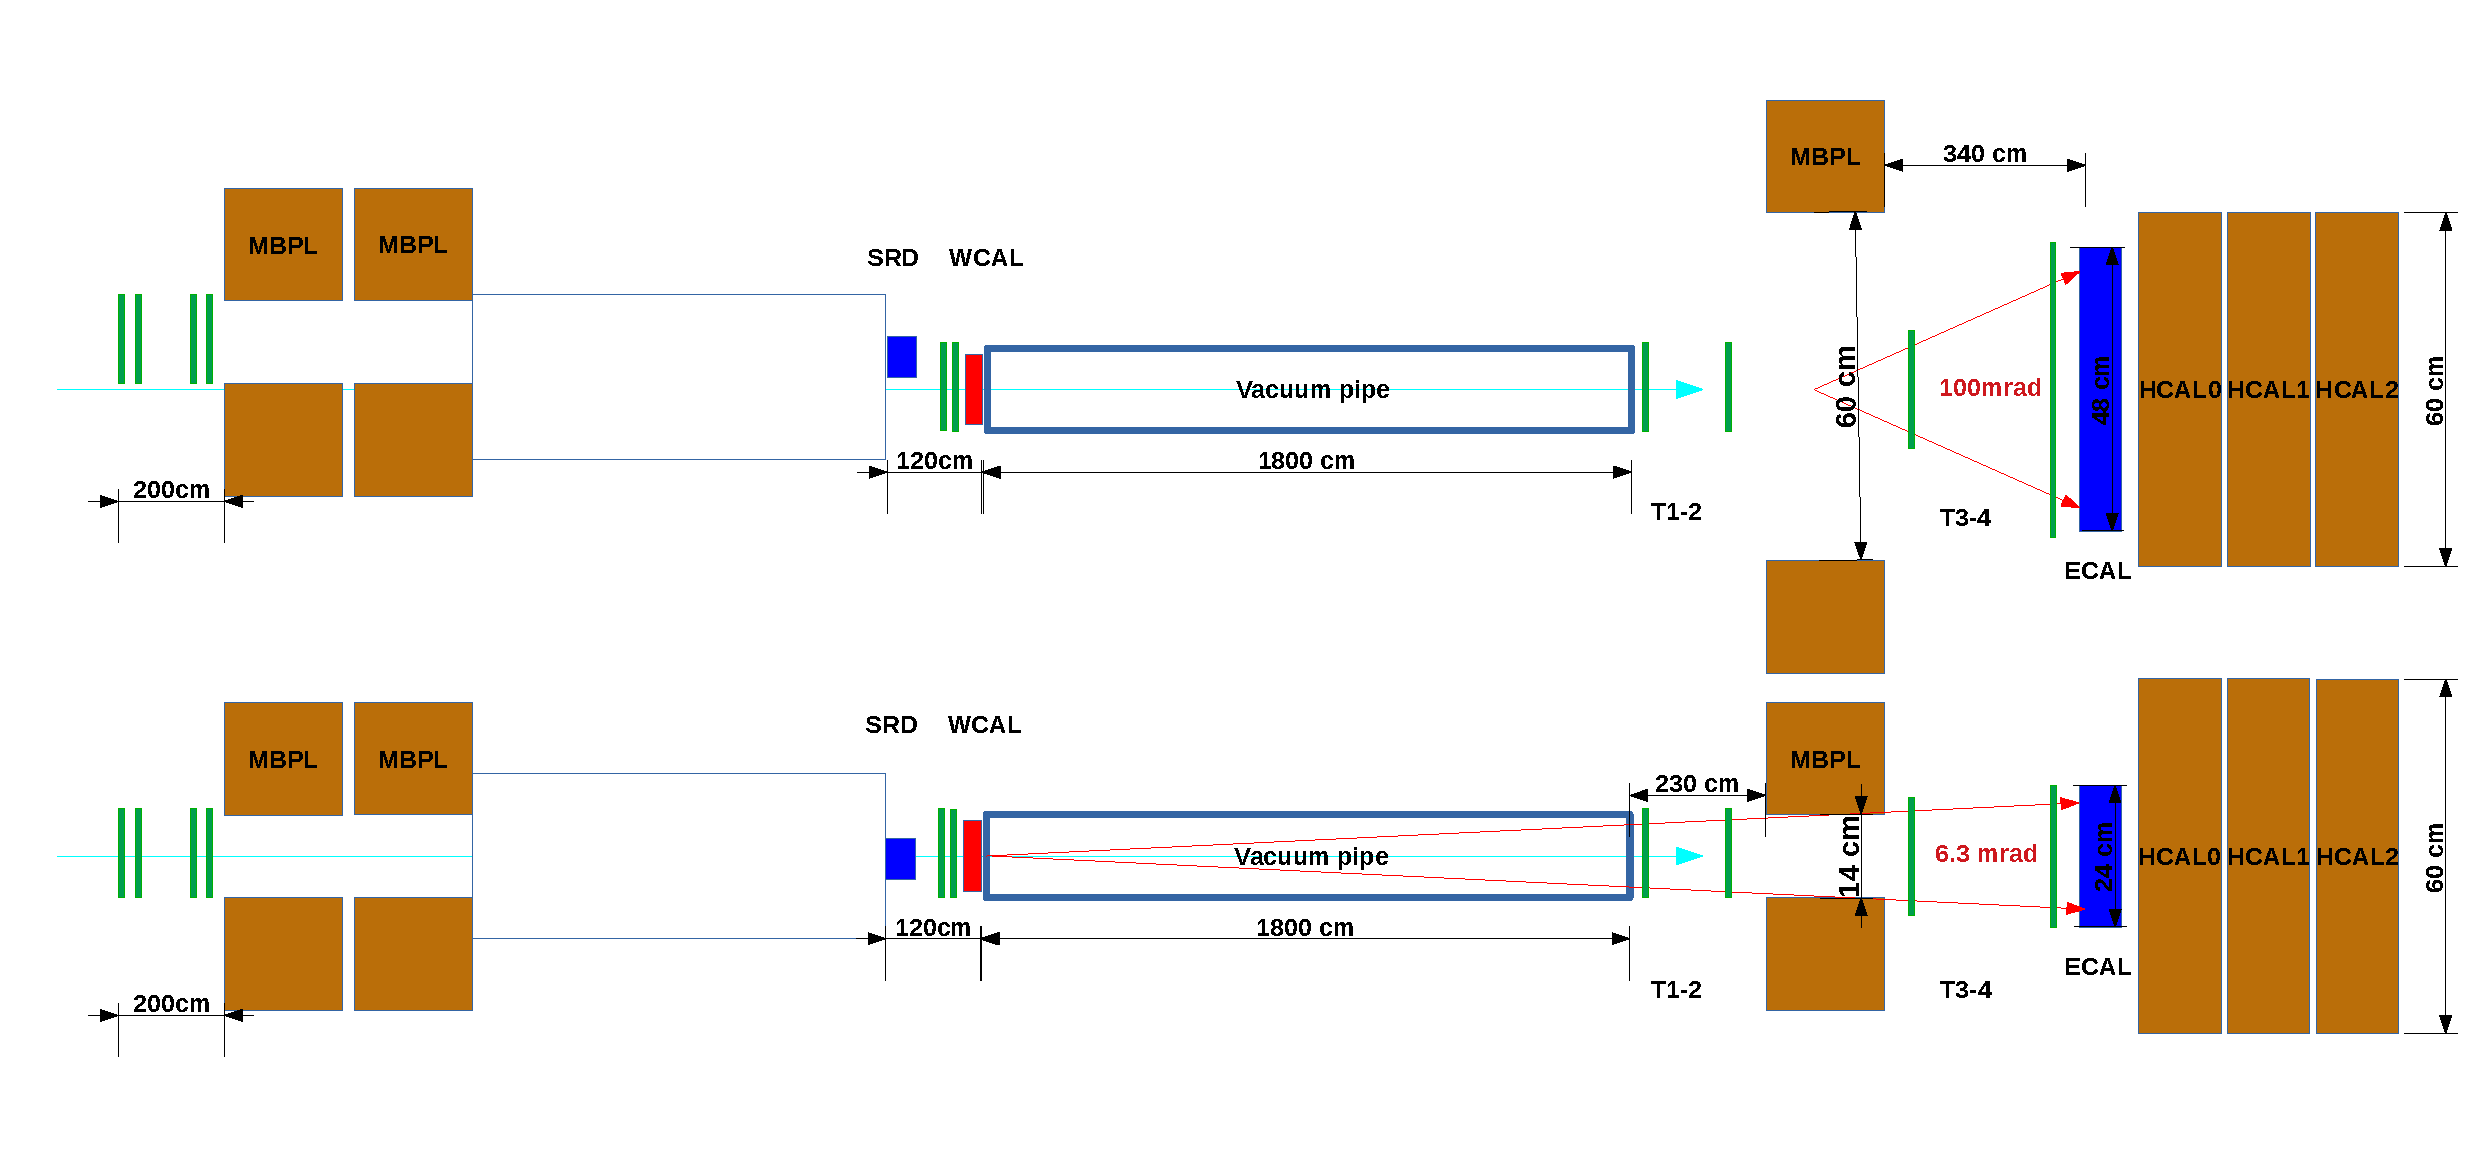
\includegraphics[scale=0.33]{\pdirfive/setup-2021.pdf}
  \caption[2021 setup]{Sketch of the setup proposed for the 2021 visible mode of NA64. Top view and side view are shown in the top and bottom pictures respectively.}
  \label{fig:setup-2021}
\end{figure}

With this scheme, the invariant mass is reconstructed with a precision of $\sim$2\% (Fig.\ref{fig:imassreco}). The fit is performed using the sum of two Gaussian functions with a shared mean corresponding to the best estimate of the invariant mass. Furthermore, 90\% of all events are reconstructed with an error smaller than 10\%. This reconstruction was performed using a MC simulation where the material budget of all detectors was reproduced precisely to estimate the impact of multiple scattering. This is detailed in the next section.

\begin{figure}[tbh!]
  \centering
  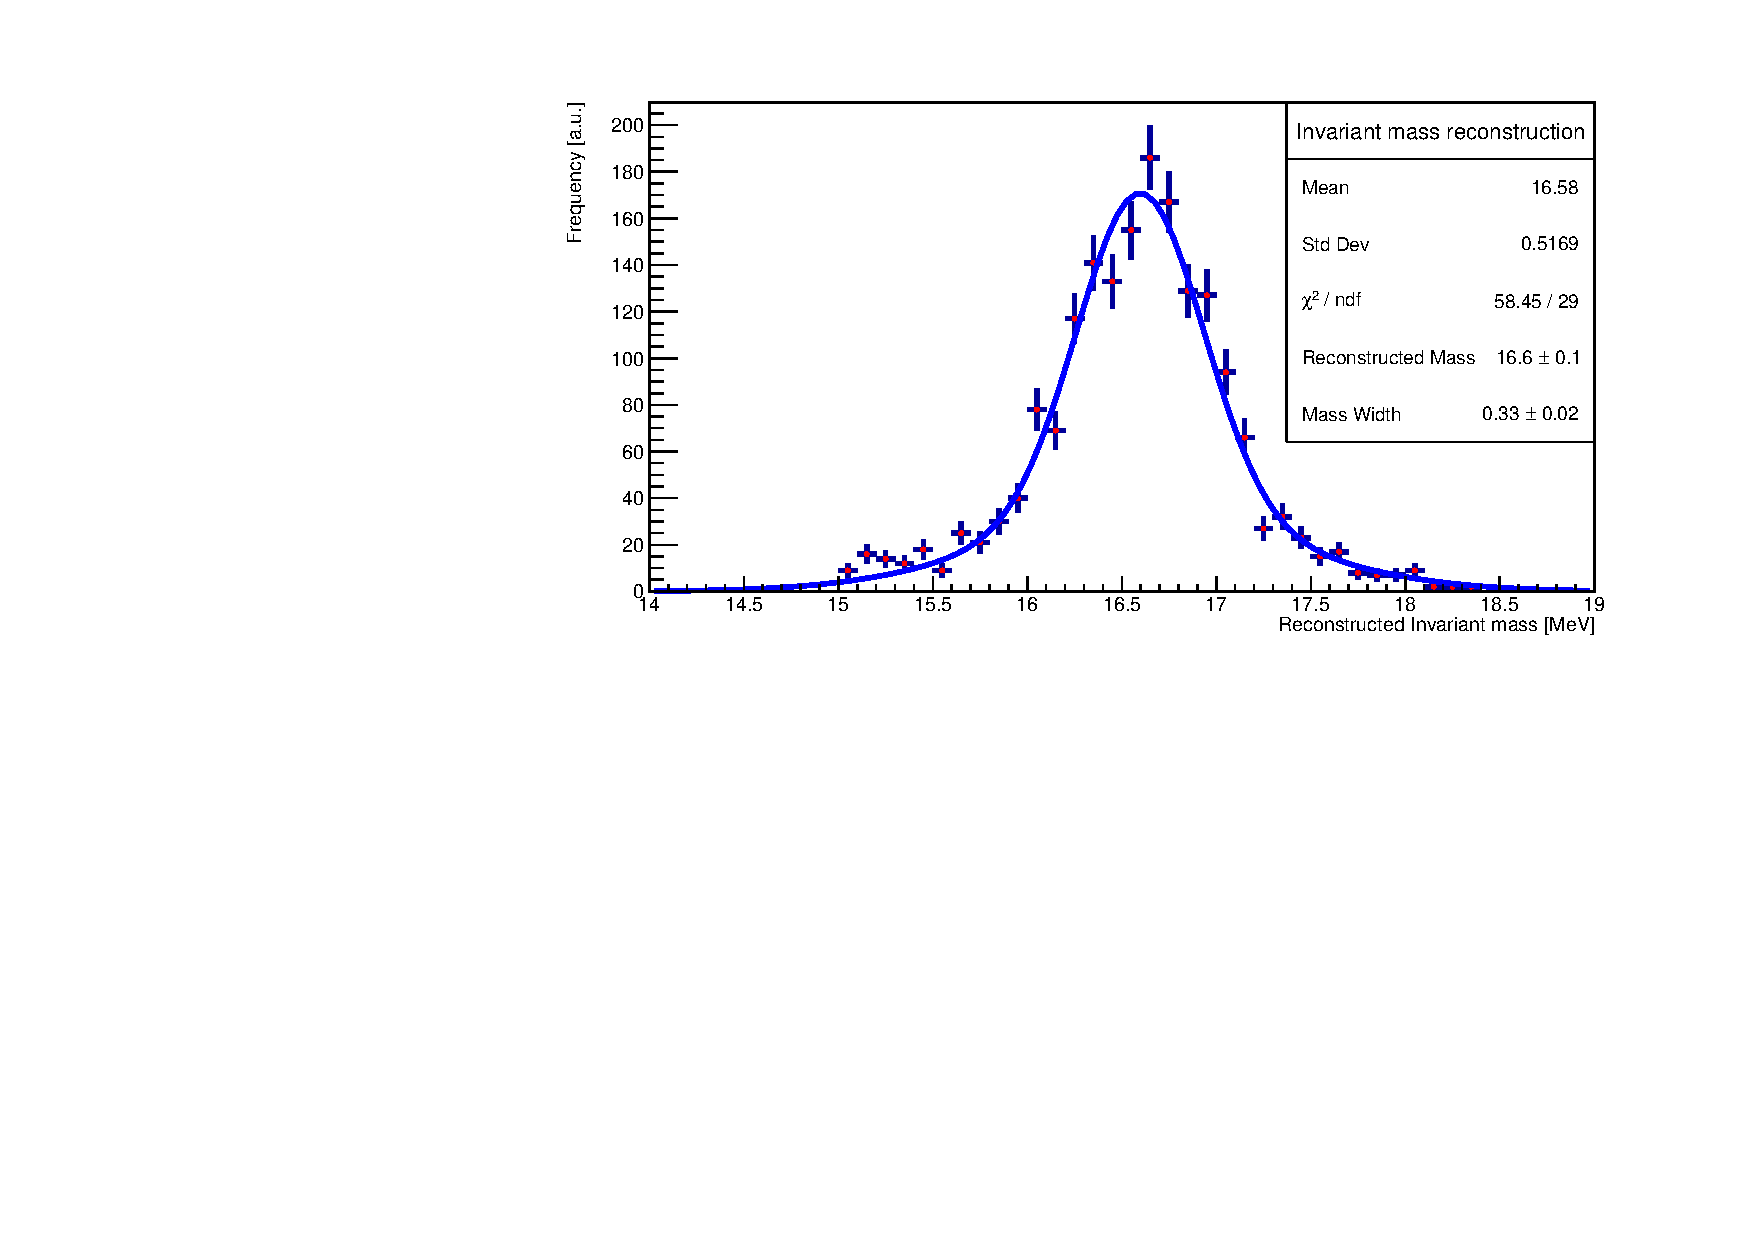
\includegraphics[scale=.8]{\pdirfive/invariant-mass-reco-allcuts.pdf}
  \caption[Invariant mass reconstruction in 2021 setup]{Reconstructed invariant mass of $\DMX$ in 2021 setup after weighting each event by its probability to decay outside the dump. 90\% of all events considered are reconstructed with 10\% precision. A fit performed with the sum of two Gaussian with the same mean is shown as a blue line. The simulation was performed using a $\DMX$ with a mass of 16.7 $\mev$ and $\epsilon = 1.4\times10^{-3}$.}
    \label{fig:imassreco}
  \end{figure}

\subsubsection{Multiple scattering effects on invariant mass reconstruction}
\label{ch5:sec:mm-scattering}

Multiple scattering experienced by the $\ee$ pair produced from the $\DMX$ decay affects the invariant mass reconstruction. As the decay takes place immediately after the dump, the multiple scattering experienced originates from:

\begin{itemize}
\item The air pocket between the end of the WCAL and the beginning of the vacuum tube.
\item The two Mylar windows are used to seal the vacuum tube.
\item \SI{18}{\meter} of low-pressure air inside the tube.
\item The air pocket between the tube and the trackers used to measure the distance of the two decay products.
\end{itemize}

Additionally, one has to consider that the thickness of W2 placed after the WCAL can also have an impact. This effect is however suppressed since most of the $\DMX$ where the decay vertex is inside the W2 are normally removed from the analysis by the requirement of a small energy deposit in this active area. The thickness of this counter was minimized from the \SI{6}{\milli\meter} used previously to \SI{3}{\milli\meter}. This reduces the contribution of multiple scattering and at the same time increases the $\DMX$ detection efficiency since the dump length is further reduced.

The vacuum tube is attached to the WCAL aluminum box to minimize the air pocket down to $\sim$1 $\mmi$. Moreover, a thin \SI{175}{\micro\meter} Mylar window is used to seal the vacuum tube which is then kept at a pressure of 8$\times 10^{-4}$ \si{\milli\bar}. The first detector is located immediately attached to the vacuum tube to reduce the air interaction to a minimum. The second Micromegas tracker is at \SI{2}{\meter} distance from the first one to compromise between angle and momentum resolution. All the materials were added in the MC simulation and their effects were studied in detail. The conclusion is that the multiple scattering has a small impact on the precision of the reconstructed invariant mass, the degradation observed compared to a scenario where only a perfect vacuum is present between the end of the WCAL and the first tracker is $\sim$0.1\%. The contributions on the invariant mass width, including limited position resolution and momentum reconstruction, are summarized in Table \ref{tab:imass-width}.

\begin{center}
  \begin{table}[bth!]
    \centering
    \begin{tabular}{|l|r|}
      \hline
      Error source & Mass width [MeV]\\
      \hline
      setup in vacuum & 0.11\\
      trackers hit resolution & 0.29\\
      vacuum window + air & 0.31\\
      momentum reconstruction & 0.33\\
      \hline
    \end{tabular}
    \caption[Error budget for the invariant mass in 2021 setup]{Width of the invariant mass after different error contributions are added cumulatively. In the first entry, all the space in the decay volume is substituted by perfect vacuum, the only material left is the one of the trackers and the W2. In the second entry, a \SI{80}{\micro\meter} hit resolution is added to the trackers. In the third entry, the vacuum is substituted by the realistic setup shown in Fig.\ref{fig:setup-2021}. Finally, the last entry add the effect of the momentum reconstruction. The invariant mass distribution with all effects considered is presented in Fig.\ref{fig:imassreco}.}
    \label{tab:imass-width}    
  \end{table}
\end{center}

\subsubsection{Hit separation in gas tracking detectors}
\label{ch5:sec:separ-hit-micr}

The NA64 experiment uses gas tracking detectors to reconstruct the incoming momentum of the electrons and reconstruct tracks in the decay volume. A set of 8 XY-multiplexed Micromegas and 4 GEM modules were employed in the invisible and visible mode setup for this purpose. As introduced in Sec.\ref{ch2:sec:vismode}, one of the main challenges of the novel setup design will be to separate two tracks at a low distance in order to reconstruct the angle of the two-body decay.

A set of clusters was extracted from the calibration data at low intensity to ensure that only single-hit were present in the considered sample. The true position of these particles was saved before randomly mixing the clusters in a new set mimicking events where two particles are hitting the trackers simultaneously. After this, a double Gaussian fit was used to extract the position of the two initial clusters, and the results of such procedure were compared to the known initial positions. The fit was performed using the Minuit2 minimizer implemented in the ROOT framework \cite{root}.

The results are summarized in Fig.\ref{fig:res-hit} where the hit resolution, defined as the mean difference between a reconstructed hit and the true one, is shown as a function of the hit separation. The part of the curve where the distance between the two clusters is between 2 and 8 strips shows a reduced hit resolution. The reason is that in this region the resulting cluster shape is significantly distorted and the fit accuracy decreases. For very close distances, on the other hand, the cluster shape converges again to the one of a single Gaussian, improving the fit result. In the specific situation of the NA64 experiment, Micromegas have a strip size of \SI{256}{\micro\meter}, which makes the two clusters separated by 9 strips ($\sim$2.3 $\mmi$). Some events with reconstructed hits exceeding a residual of 1 $\mmi$ can be found for a separation smaller than 10 strips. These hits are typically caused by some abnormal cluster topology that breaks the Gaussian assumption used by the fit. For hits with separation larger than 2 $\mmi$ no such events are observed. In the setup proposed, the minimum distance between the decay products is 3 $\mmi$ as shown in Fig.\ref{fig:dm_dist1}. As the separation of the decay products is predicted to be much larger than the distance where the two clusters are completely separated, the detection efficiency of the $\DMX$ is not reduced by the reconstruction of the hits, and is only limited by the detector efficiency ($\sim$98\% for a single primary \cite{Banerjee:2017mdu}).

\begin{figure}[tbh!]
  \centering
  %%%
  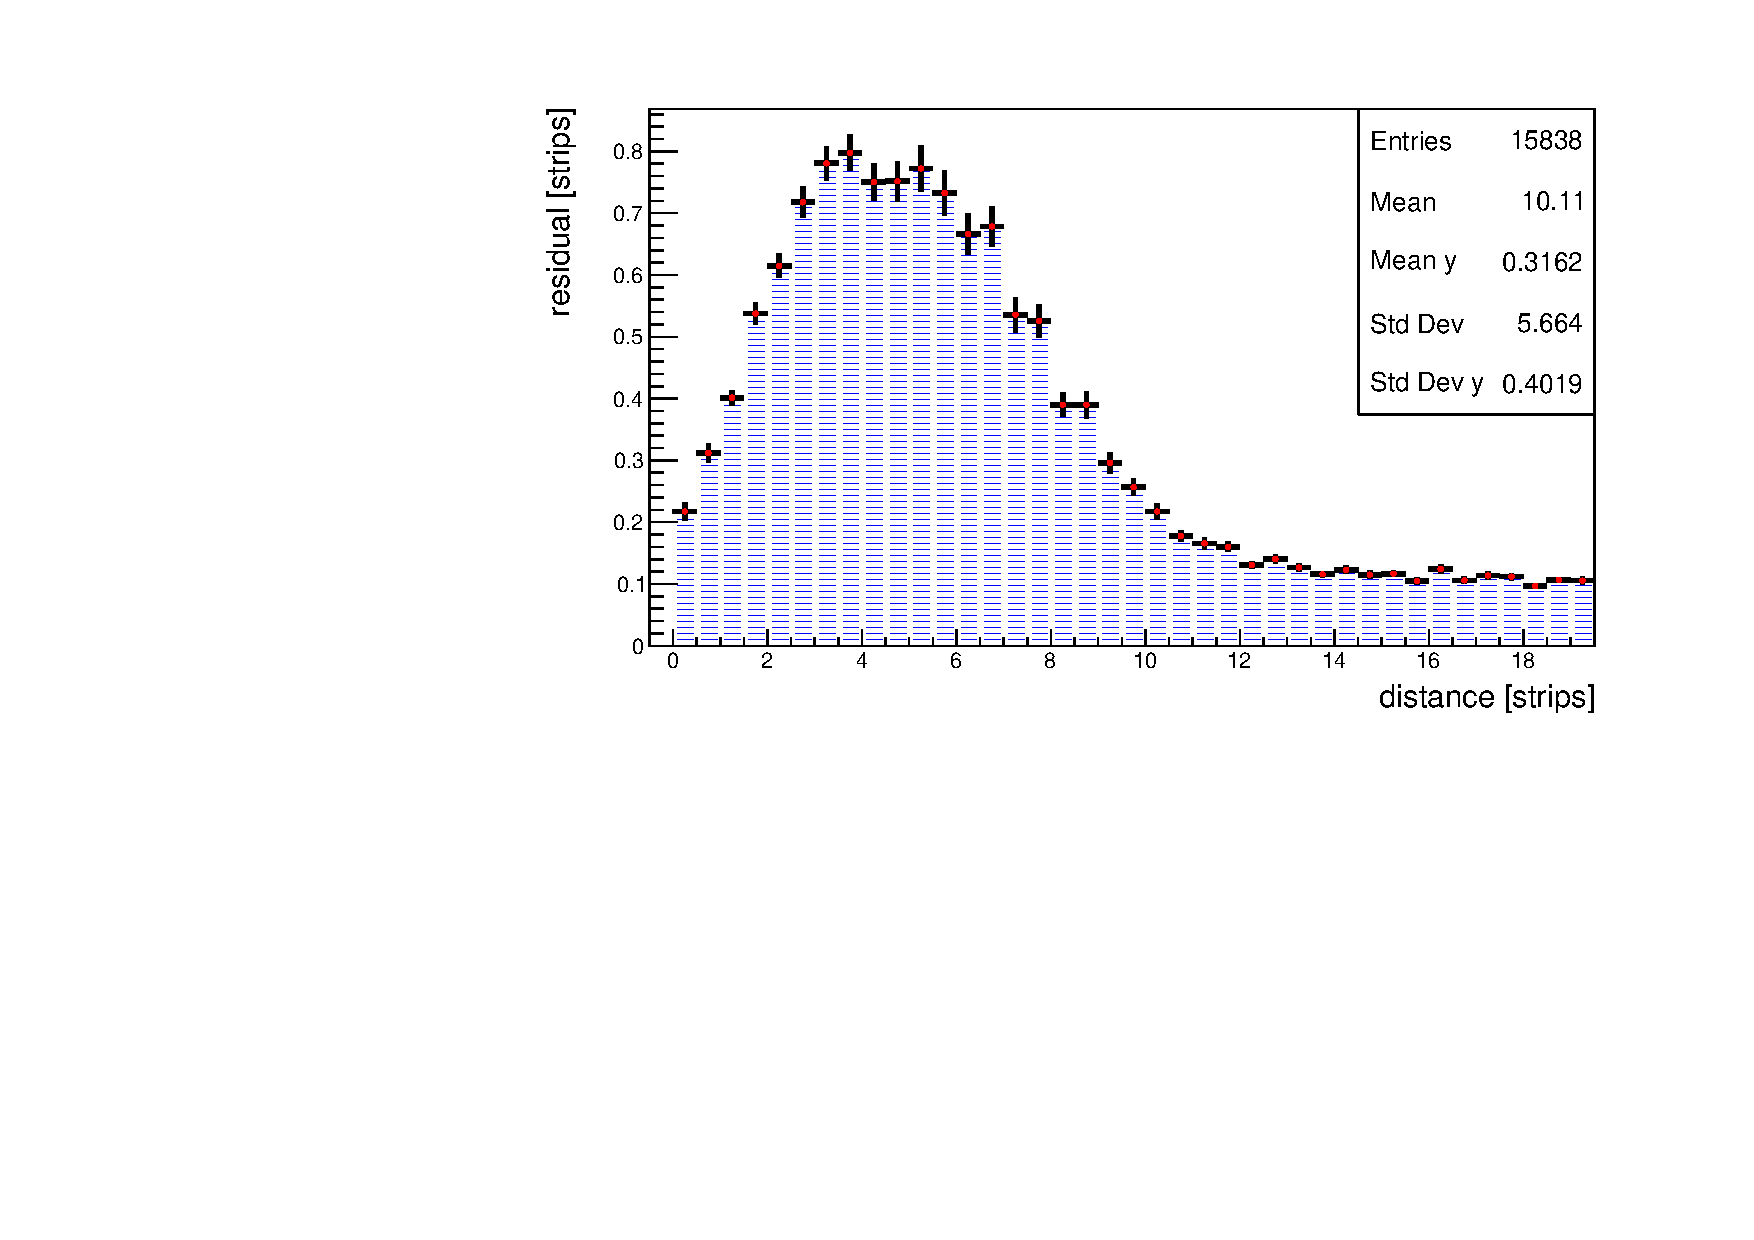
\includegraphics[width=\textwidth]{\pdirfive/res.pdf}
  \caption[Hit resolution as function of the two cluster distance]{Hit resolution of two separate clusters in a same plane as function of the distance between the two. The units are given in strips size, where a single strip has a size of \SI{256}{\micro\meter} for the Micromegas used in the NA64 experiment.}
  \label{fig:res-hit}
\end{figure}

\subsection{WCAL optimization}
\label{ch5:sec:new-vismode-setup-wcal}

To boost the signal yield for the $\DMX$ we need to increase its probability of decaying outside the target. We see from Eq.\ref{eq:dm-decay-length} that this number scales linearly on both the nominal energy of the beam and the dimension of the dump. In 2018, the energy was already increased to 150 $\gev$ to boost this probability. Additional raise in energy will have several demerits: larger background from hadron contamination in the beam decreased flux and a shorter bending that would reduce the SRD rejection power. Instead, a new design of the WCAL with a short longitudinal dimension can achieve the same purpose while keeping the background under control.

To design the new calorimeter structure, the figure of merit is the signal efficiency, which is defined mostly by the number of $\DMX$ that decay outside the WCAL. This was quantified by a detailed MC-simulation used to generate the energy spectrum and the decay kinematics of the $\DMX$.

In the design used in previous searches, the WCAL had 34 layers in total, each of them consisting of a converter layer made of 3 mm of Tungsten and an active part made of a 2 mm plastic scintillator. This sums to a total of $\sim$30X$_0$. Reducing the dimension of the WCAL would impact the radiation length used to contain the main shower and hence change the background conditions. To avoid this, the new design was studied under the principle that the optimal radiation length should be approximately 30X$_0$. Three different versions were considered:

\begin{itemize}
\item An initial part of 9 layers using the original layer structure followed by an additional 25 layers of only tungsten.
\item A calorimeter consisting of 17 layers with layer-structure: 6mm tungsten + 2mm plastic scintillator.
\item A calorimeter consisting of 12 layers with a different structure: 9mm tungsten + 2mm plastic scintillator.
\end{itemize}

In all designs, the initial 5 layers forming the pre-shower part are still used for efficient hadron rejection. Despite its longer length, the first design grants a good energy resolution and a good hermeticity. In the second and third cases, the calorimeter is more compact but has a worse energy resolution due to the thicker converter. A sketch of the two last designs is shown in Fig.\ref{fig:wcal-design} and compared to the original one used in the previous search.

The third design was chosen to be the most suited for our experiment. The loss in energy resolution has almost no impact on the signal efficiency. The reason is that the short lifetime of the $\DMX$ favors the detection of the ones produced at high energy that are able to escape the dump more efficiently. These $\DMX$ carry most of the initial e$^-$ energy outside of the WCAL and its decay is detected in the downstream (ECAL). Hence, the energy is reconstructed with a precision of $<$1\% regardless of the WCAL structure. The second and third designs are compared to the original WCAL in Table \ref{tab:wcal-length-results}.

\begin{center}
\begin{table}[tbh!]
  \begin{tabular}{|lcr|}
  \hline
  WCAL structure [mm](layers)  & $\epsilon$  & EOT to cover $\DMX$ at 90\% confidence [$10^{10}$] \\
  \hline
  ECAL1:3+2(34)                & 0.001   & 17$\pm$3.4                                            \\ 
  ECAL1:6+2(17)                & 0.001   & 7$\pm$0.9                                             \\
  ECAL1:9+2(12)                & 0.001   & 6$\pm$0.7                                             \\
  ECAL1:3+2(34)                & 0.0012  & 85$\pm$4.7                                            \\
  ECAL1:6+2(17)                & 0.0012  & 24$\pm$6.9                                            \\  
  ECAL1:9+2(12)                & 0.0012  & 19$\pm$5                                              \\  
  \hline
\end{tabular}
\caption[Possible WCAL designs and  their projected experimental reach]{Number EOT required to cover $\DMX$ at 90\% confidence using different WCAL designs in the visible mode setup proposed for 2021. The first entry describes the structure using the convention:
  ECALconverter-depth+counter-depth(number-of-layers).}
\label{tab:wcal-length-results}
\end{table}
\end{center}

\begin{figure}[tbh!]
  \centering
  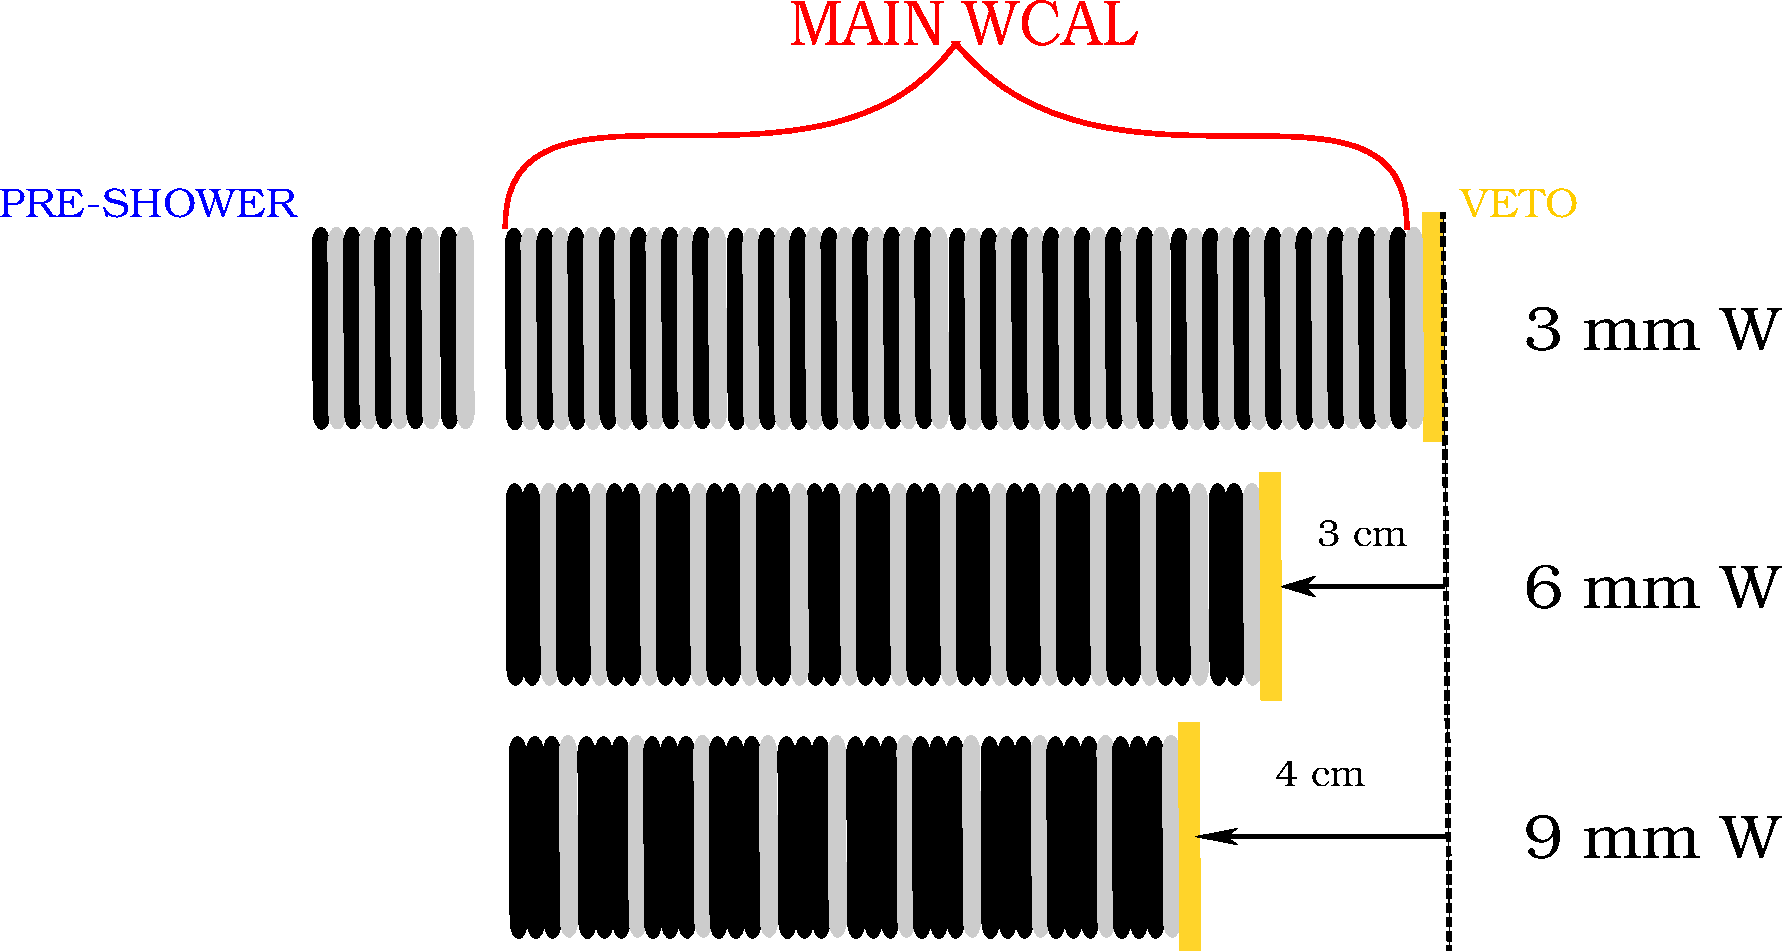
\includegraphics[scale=0.5]{\pdirfive/WCAL_design.pdf}
  \caption[New WCAL design for 2021]{Possible designs of the WCAL re-arranging the available tiles of 3 $\mmi$ of Tungsten (W) and 2 $\mmi$ of scintillator material. All designs posses the same radiation length of 30$X_0$.}
  \label{fig:wcal-design}
\end{figure}


\subsubsection{Background and sensitivity}
\label{ch5:sec:background-sensitivity}

A preliminary study of the background was performed in this novel setup. As discussed in chapter \ref{chapter3} the main source of background is coming from the production of $\ks$ in the WCAL escaping the dump and decaying in the vacuum tube as the $\DMX$. The decay products can potentially mimic the signal either in the chain K$^0_S \rightarrow \pi^0 \pi^0$ where $\ee$ pair are produced in the $\gamma$ conversion of the photon pair into an $\ee$ or in the rare decays $\pi^0 \rightarrow \gamma e^- e^+$. To estimate the impact of such a background simulation of 5$\times 10^6$ $\ks$ was performed using the energy spectrum expected from the production of this particle via electro-nuclear interactions.
The conservative assumption of the simulation is that the $K^0_S$ is produced in an inelastic scattering in the WCAL where all the energy is deposited inside the dump without leaving a significant signature in W2. It was found that only 3\% of the events left a shower separation in the ECAL similar to the one expected from $\DMX$. Less than 1\% of the events are within the acceptance of the trackers. In the majority ($>$90\%) of the surviving events, the $\ks$ has an energy $<$60 \gev. This spectrum is significantly different from the one predicted for the $\DMX$, where 95\% of the spectrum is above 100 \gev with a sharp peak at 150 \gev (the nominal beam energy). Finally, no event in the sample was reconstructed with an invariant mass compatible with the $\DMX$, the closest one being reconstructed at 280 MeV. This is well above any $A'$ scenario in reach of the NA64 experiment \cite{Banerjee:2019hmi}. As the new WCAL design conserves the hermeticity of 30$X_0$, the background coming from $\gamma$-punchtrough is not expected to increase in the new setup. This contribution is hard to study in detail using MC simulation, it was however demonstrated in our previous measurements \cite{Banerjee:2019hmi} that a longer setup adds a suppression to this contribution due to the longer decay volume. As both neutral-punchtrough and $\ks$ are not expected to increase, one can conservatively put the background at a level of $<0.01$ (see Table \ref{tab:vis-bkg}).

An analysis based on the simulated data was conducted to estimate the reach of the experiment using the proposed setup. Most of the selection criteria already applied in our previous searches were used for this study. Additionally, a separation of at least 8 cm (for a cell size of dimension 38$\times$38 $\mms$) is required between the two electromagnetic showers and the reconstructed invariant mass is selected to be within 10\% of the expected $\DMX$ mass. The expected signal yield was computed after all the cuts were applied and used to calculate the 90\% sensitivity for different $\DMX$ scenarios. The results of the computation are presented in Fig.\ref{fig:exclusion-x17} that shows the number of EOT necessary to probe a specific $\DMX$ scenario. Assuming a trigger-rate similar to the one observed during 2018 visible-mode data taking, a projection of the days needed is also shown. As expected, the EOT required to probe a specific $\DMX$ model increases exponentially with the coupling strength $\epsilon$, since the signal yield is dominated by the probability of $\DMX$ to exit the dump. The conclusion is that the complete range $\epsilon < 1.4 \times 10^{-3}$ of $\DMX$ parameter space proposed in \cite{PhysRevD.95.035017} can be covered in approximately 3 months of beam time by accumulating $\sim 7 \times 10^{11}$ EOT. Models with V$\pm$A coupling mentioned in Sec.\ref{ch1:sec:dm-candidates} on the other hand can be covered faster ($<$10 days) due to the smaller allowed coupling. 

\begin{figure}[htb!]
  \centering
  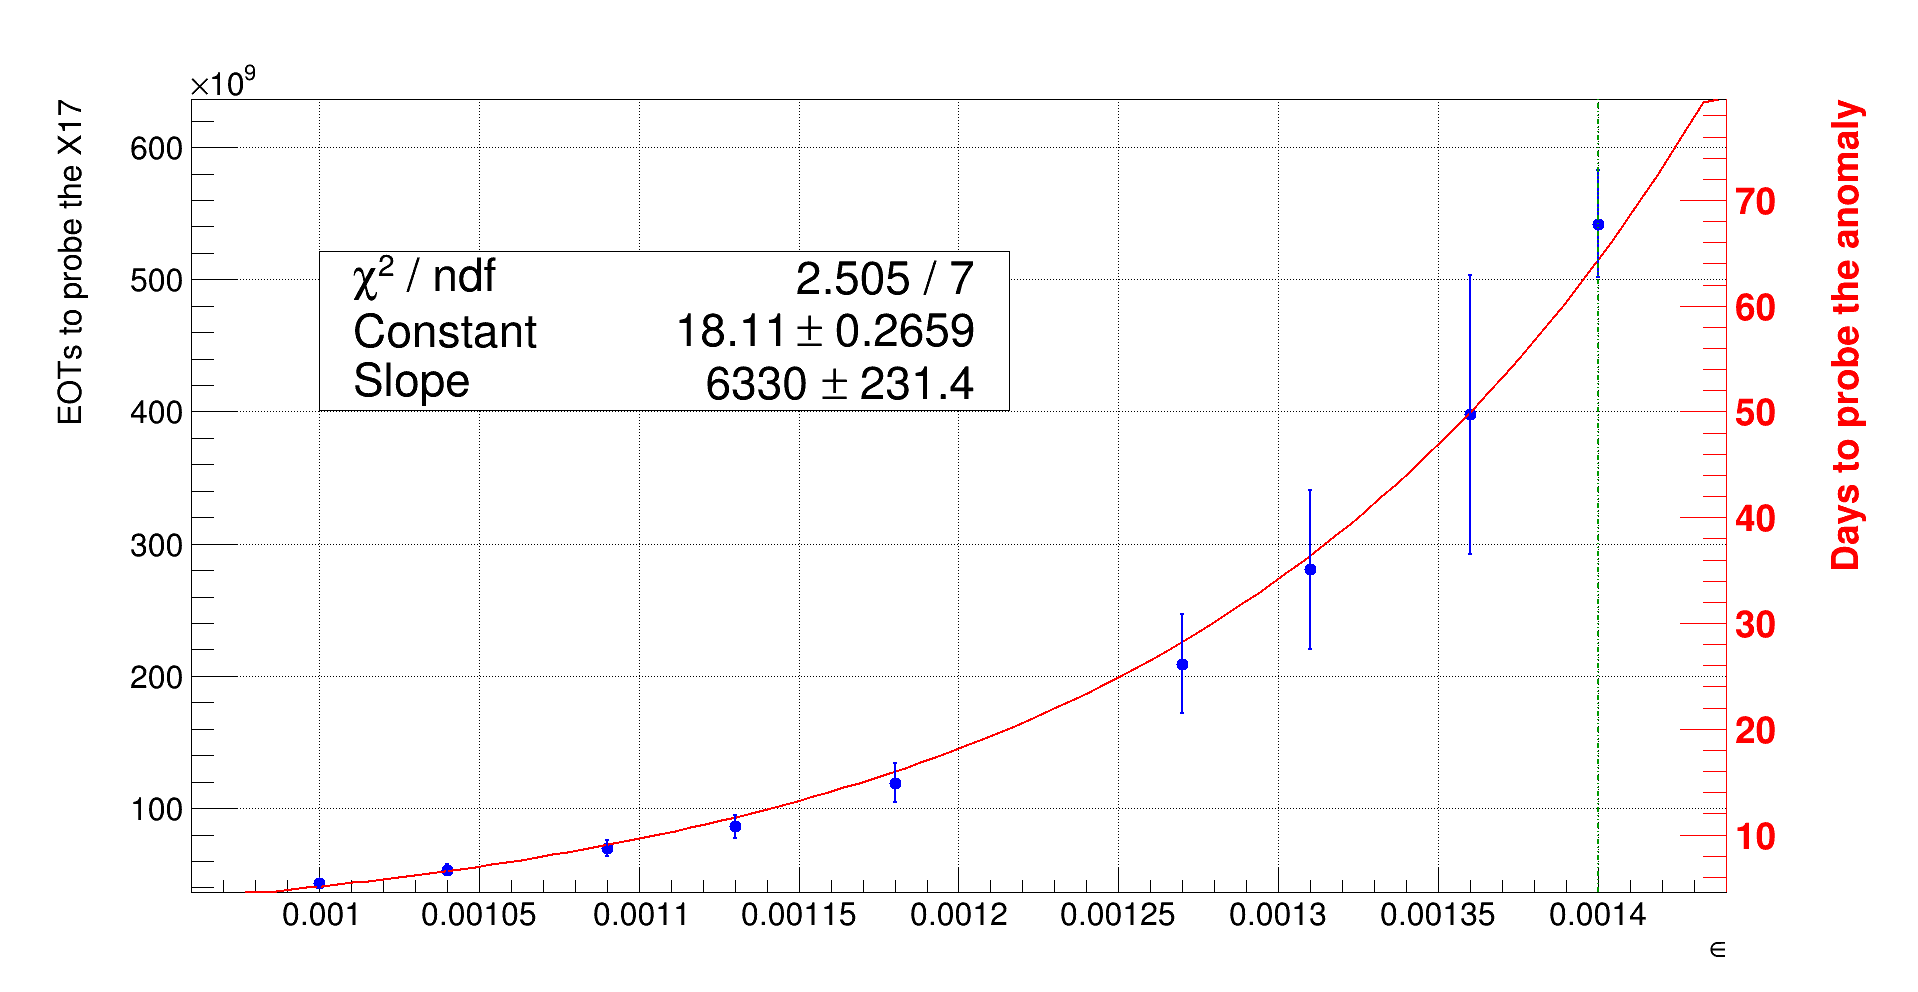
\includegraphics[width=\textwidth]{\pdirfive/exclusion_167_exclusion.png}
  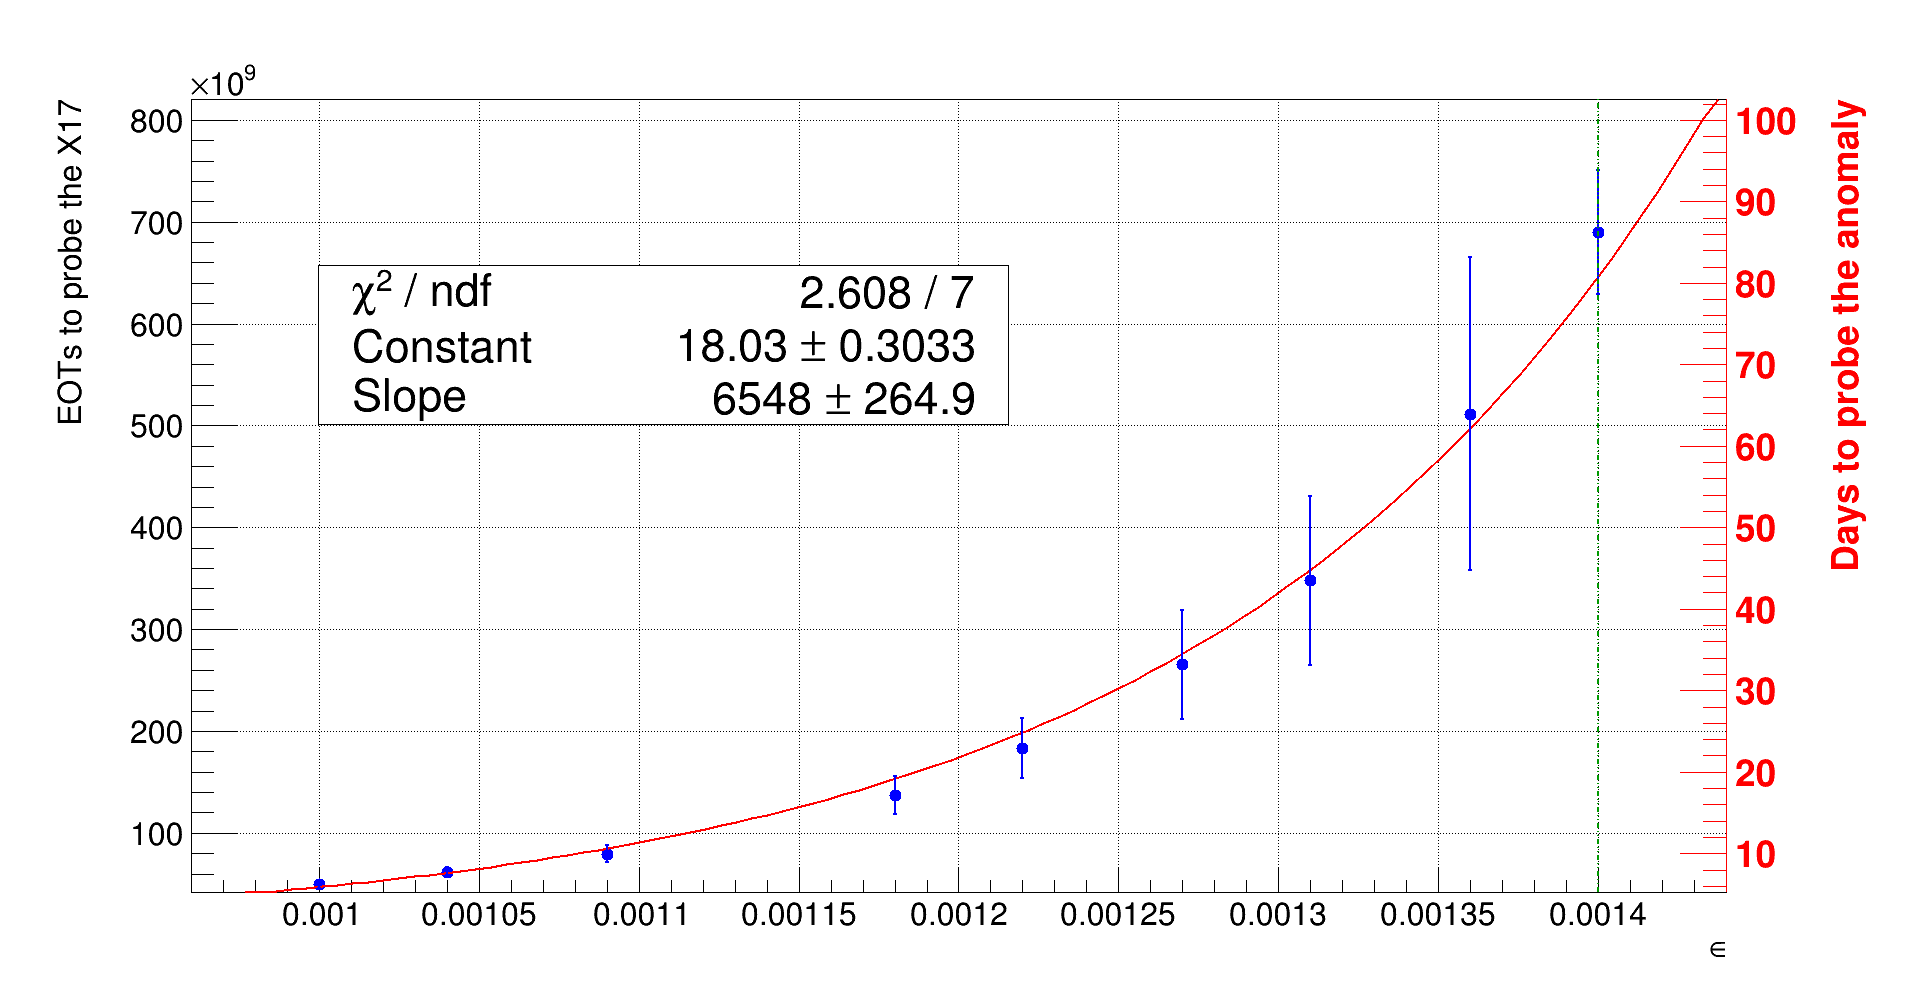
\includegraphics[width=\textwidth]{\pdirfive/exclusion_170_exclusion.png}
  \caption[EOT to X17 exclusion]{Number of EOT needed to probe the $\DMX$ with an exclusion limit of 90\% assuming negligible background as a function of $\epsilon$ on the left y-axis, while the number of days required to accumulate the correspondent number of EOT is shown in the right y-axis and is based on the trigger-rate measured during the 2018 visible mode data taking \cite{Banerjee:2019hmi}. The green dashed line shows the maximum $\epsilon$ permitted if $\DMX$ is interpreted as protophobic gauge boson \cite{PhysRevD.95.035017}. The detection efficiency for high $\epsilon$ is dominated by the probability of $\DMX$ to exit the dump as it is shown by the exponential fit (red line). The plot is shown for the two most relevant mass scenarios suggested by the two experiments conducted by the ATOMKI group, i.e. 16.7 MeV (top) and 17.0 MeV (bottom) \cite{Krasznahorkay:2015iga,Krasznahorkay:2019lyl}.}
  \label{fig:exclusion-x17}
\end{figure}
  
\FloatBarrier\noindent
\section{A new approach: the Muon mode setup}
\label{ch5:sec:muon-mode-setup}

A new approach proposed for the next generation of fixed-target experiments performed by the NA64 collaboration is to use a muon beam instead of an electron one. This search would boost the sensitivity for $\DM$, in particular for a dark mediator mass $m_{\DM} \gtrsim 100 \mev$ as suggested by a detailed calculation performed using the ETL cross-section \cite{Gninenko:2019qiv}. Additionally to the boost in the sensitivity for the $\umodel$, this setup would be sensitive to a dark mediator weakly coupled to muon. One example of such a particle would be a $\DMU$ which interacts predominantly via a $L_{\mu} - L_{\tau}$ current \cite{krasnikov2017muon,GNINENKO2001119}. Other appealing properties of this mediator include a mechanism to account for the observed DM relic abundance \cite{GNINENKO2001119,Kirpichnikov:2020tcf,PhysRevLett.121.011102} and the $\ammu$ anomaly. This is also possible in the case of a muon-specific scalar mediator \cite{krasnikov2017light,PhysRevD.95.115005}.

This new experiment will use the M2 muon beamline which provides 160 \gev muons at a rate of a few 10$^7$ (Muon On Target) MOT per spill. The setup will be placed upstream of the COMPASS experiment, in a space of \SI{13}{\meter}. The case of a muon beam differs significantly from the electron case previously studied. Nevertheless, "Dark-Bremsstrahlung" is still the primary production channel:

\begin{equation}
  \label{eq:dm-muon-int}
  \mu + Z \to Z + \DMU + \mu
\end{equation}

Because of the higher penetration power of the muon, the interaction can happen along the full length of the target, and not mainly in the first few radiation lengths as in the case of an electron primary.
For a mass larger than 100 \mev, the expected decay time for this particle is of the order of $\tau_{\DMU} \lesssim 10^{-15} \si{\second}$. Thus, its decay is expected inside the setup shortly after its production. For a mass $M_{\DMU} > 2 m_{\mu}$ the branching ratio is evenly shared between the invisible channel $\DMU \to \nu \bar{\nu}$ and the visible channel $\DMU \to \mu^+ \mu^-$. The latter corresponds to a muon-trident signature and is not currently considered for the analysis due to the high background from the dimuon production $\gamma \to \mu^+ \mu^-$. The current design focuses on the invisible channel, hence the signature is missing momentum. To measure the energy of the $\mu^-$ primary after the interaction, a calorimeter approach is not feasible as this particle cannot be reliably stopped inside the dump. Instead, a second magnetic spectrometer is placed after the target to tag the scattered muon and measure its momentum again. The total energy deposited inside the ECAL must be compatible with the one of a single MIP passing through the detector, to make sure that no energy was lost because of Bremsstrahlung radiation or nuclear interaction. A two weeks pilot run to test the feasibility of the technique has been approved by the CERN SPSC and is foreseen by the end of 2021. The setup is constructed by rearranging the detectors already used in the experiments using the electron beam. The ECAL is placed immediately after a first magnetic spectrometer (MS1), while the HCAL modules are located $\sim$6 \si{\meter} downstream after the second spectrometer (MS2) to detect the scattered muon. To reduce background from large nuclear interactions inside the ECAL, the VHCAL module discussed in Sec.\ref{ch5:sec:new-invismode-setup} is placed after MS2 to catch particles emitted at large angles. A sketch of the proposed setup is illustrated in Fig.\ref{fig:muon-mode-setup}.

The experiment also needs an alternative method to reduce the initial trigger rate that does not rely as in the electron mode on the energy deposited inside the calorimeters. A set of scintillator counters is used for this purpose:
\begin{itemize}
\item $S_0$ and $S_1$: characterize the beam.
\item $V_{m1}$,$V_{m1}$,$V_{m3}$,$V_{m4}$:  are used to reject low energy particles entering the magnets.
\item $S_4$: A scintillator counters shifted 5 \si{\centi\meter} away from the beam axis triggers the deflected muons.
\item $V_1$: is used to veto the primary beam to avoid a fake trigger of $S_4$ caused by the production of secondaries along the beamline.
\item $S_{\mu}$: tag the scattered muons penetrating the four HCAL modules.
\end{itemize}

The trigger condition combines all the information of these detectors:

\begin{equation}
\label{eq:trigger-mumode}
Tr^{\DMU} = S_0 \times S_1 \times \overline{V_1} \times \overline{V_{m1}}\overline{V_{m2}}\overline{V_{m3}}\overline{V_{m4}}\times S_{\mu}
\end{equation}

\begin{figure}[bth!]
  \centering
  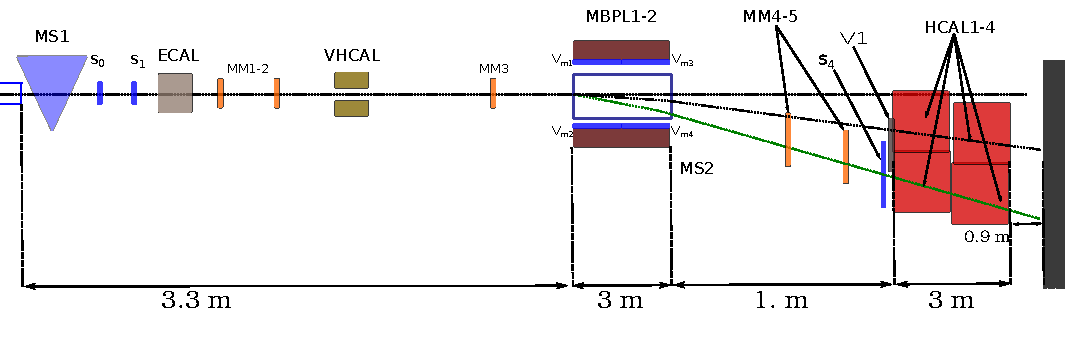
\includegraphics[width=\textwidth]{\pdirfive/setup-muon-2021.pdf}
  \caption[Sketch of muon mode setup 2021 for phase 1]{Scheme of 2021 muon mode setup. In Green the direction of a muon scattering in the ECAL is shown.}
  \label{fig:muon-mode-setup}
\end{figure}

The selection criteria are chosen to tag only muons that did not have a hard-scattering inside the ECAL. Hence, less than 1 $\gev$ energy deposit in the VHCAL and less than 4 $\gev$ energy in each HCAL module are required. Only events with reconstructed momentum compatible with 160 \gev are selected as candidates. Events are binned in the plane (E$_{ECAL}$ + E$_{HCAL}$; p$_{\mu}$), where p$_{\mu}$ is the momentum reconstructed in MS2. The signal region is then defined as p$_{\mu} <$80 $\gev$ and (E$_{ECAL}$+E$_{HCAL}$) $<$ 20 $\gev$. This means that to be selected a muon must have lost at least half of its original energy without any significant energy deposit in any of the calorimeters placed along the beamline.

A detailed MC-simulation developed by me and other ETH group members was used to test the feasibility of the setup. The goal was to assess the sensitivity of the test-beam setup in a realistic scenario. The number of MOT which could be accumulated during the pilot run and the possible background sources were estimated. The beam profile used as input for this simulation was extracted using a dedicated simulation provided by the beam CERN department to reproduce faithfully the interaction along the beamline. It was found that the expected background, mostly caused by large scattering neutrals produced in the ECAL, is at the level of $\lesssim 10^{-11}$. 

The setup will be tested in 2021 and a first physics run is planned for 2022, in the so-called phase 1, where the $\ammu$ parameter space will be probed by accumulating 10$^{11}$ MOT. The setup for Phase 2 is shown in Fig.\ref{fig:muon-mode-setup-phase2}. The main differences with respect to the pilot run are a second spectrometer consisting of two MBPL magnets to improve the scattered muon measurement, a second VHCAL between the two magnets, and a larger HCAL to improve hermeticity and reach a background level of $10^{-13}$ MOT. $NA64_{\mu}$ plans a second phase after LS3\footnote{Long Shutdown 3 of the LHC}, where $\sim 10^{13}$ MOT will be accumulated to gain sensitivity on the parameter space justifying the observed relic abundance of Dark Matter \cite{Gninenko:2640930}. The projected sensitivities in the second phase, combined with the expected electron results are illustrated in Fig.\ref{fig:dmyplane-mumode}.

\begin{figure}[bth!]
  \centering
  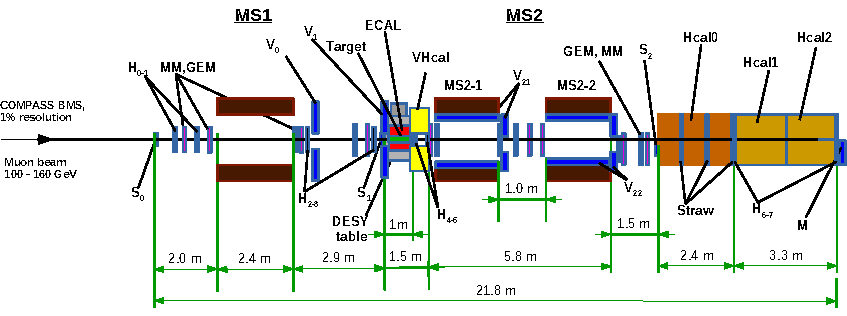
\includegraphics[width=\textwidth]{\pdirfive/setup-muon-2022.pdf}
  \caption[Sketch of muon mode setup 2022 for phase 1]{Sketch of muon mode setup 2022 \cite{Gninenko:2640930}.}
  \label{fig:muon-mode-setup-phase2}
\end{figure}

\begin{figure}[bth!]
  \centering
  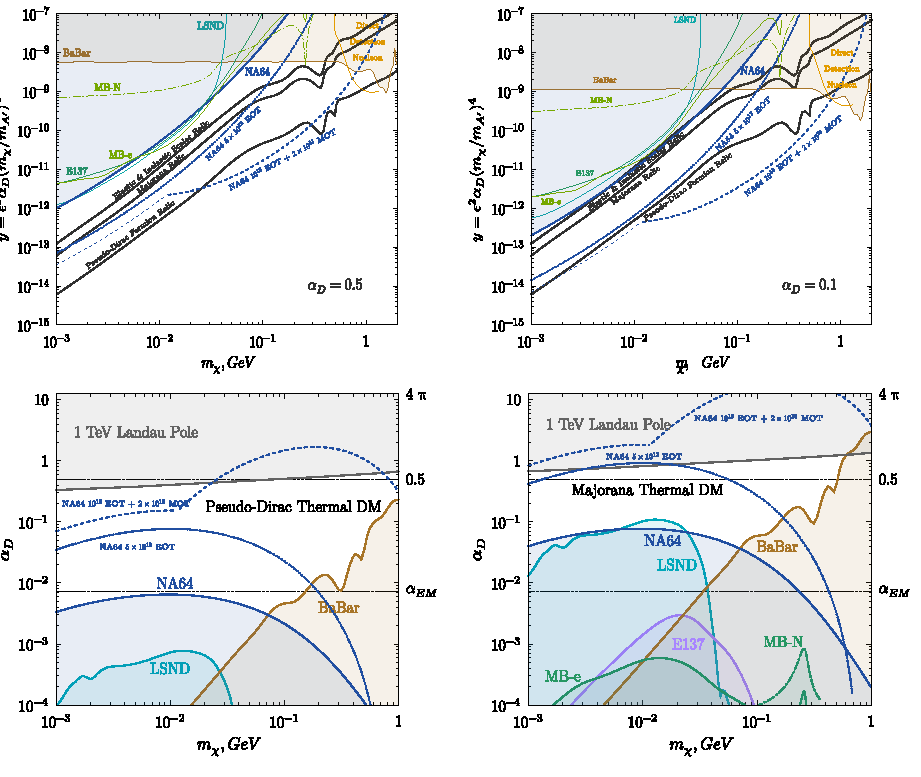
\includegraphics[width=\textwidth]{\pdirfive/tldra-21-1-mumode.pdf}
  \caption[sensitivity projection for invisible mode + muon mode 2021]{Projection of sensitivity of the NA64 experiment in the $\dmyplane$ for $5 \times 10^{12}$ EOT and for $5 \times 10^{12}$ EOT + $2 \times 10^{13}$ MOT that will are planned to be collected after LS3 \cite{Gninenko:2019qiv}.}
  \label{fig:dmyplane-mumode}
\end{figure}

%%% Local Variables:
%%% mode: latex
%%% TeX-master: "../PhDthesis"
%%% End: